\documentclass[serif,mathserif,final]{beamer}
\mode<presentation>{\usetheme{Lankton}}
\usepackage{amsmath,amsfonts,amssymb,breqn,times,pxfonts,xspace}
\usepackage{graphicx}
\usepackage{color}
\graphicspath{{../figures/}}
\usepackage[orientation=landscape,size=custom,width=70,height=40,scale=.6,debug]{beamerposter}

%%%%%%%%%%%%%%%%%%%%%%%%%%%%%%%%%%%%%%%%%%%%%%%%%%%%%%%%%%%%%%%%%%%%%
% Macros
%%%%%%%%%%%%%%%%%%%%%%%%%%%%%%%%%%%%%%%%%%%%%%%%%%%%%%%%%%%%%%%%%%%%%
\newcommand\seteq{\mathrel{\overset{\makebox[0pt]{\mbox{\normalfont\tiny\sffamily set}}}{=}}} % equality with the text "set"
\newcommand\bbR{\ensuremath{\mathbb{R}}} % Real numbers
\newcommand\bbZ{\ensuremath{\mathbb{Z}}} % Integers
\newcommand\bbE{\ensuremath{\mathbb{E}}} % Expectation
\DeclareMathOperator*{\tr}{tr} % Trace
\DeclareMathOperator*{\diag}{diag} % Diagonal matrix
\DeclareMathOperator*{\sign}{sign} % Sign
\DeclareMathOperator*{\var}{Var} % Variance
\DeclareMathOperator*{\cov}{Cov} % Covariance
\newcommand{\1}{\mathbb{I}} % Indicator
\DeclareMathOperator*{\argmax}{arg\,max} % argmax
\DeclareMathOperator*{\argmin}{arg\,min} % argmin
\DeclareMathOperator*{\minimize}{minimize} % minimize
\DeclareMathOperator*{\maximize}{maximize} % maximize

%%%%%%%%%%%%%%%%%%%%%%%%%%%%%%%%%%%%%%%%%%%%%%%%%%%%%%%%%%%%%%%%%%%%%
% Custom Beamer Setting
%%%%%%%%%%%%%%%%%%%%%%%%%%%%%%%%%%%%%%%%%%%%%%%%%%%%%%%%%%%%%%%%%%%%%
\setbeamertemplate{caption}[numbered]
\setbeamertemplate{itemize/enumerate body begin}{\normalfont}
\setbeamertemplate{itemize/enumerate subbody begin}{\smallfont}
\setbeamertemplate{itemize/enumerate subsubbody begin}{\smallfont}
\setbeamertemplate{bibliography item}[numbered]

%-- Header and footer information ----------------------------------
\newcommand{\footleft}{}
\newcommand{\footright}{Christopher B. Choy\textsuperscript{\dag}, Michael
  Stark\textsuperscript{\ddag}, Sam Corbett-Davies\textsuperscript{\dag},
  Silvio Savarese\textsuperscript{\dag}}
\title{Enriching Object Detection with 2D-3D Registration and Continuous
  Viewpoint Estimation}
\author{Christopher B. Choy\textsuperscript{\dag}, Michael
  Stark\textsuperscript{\ddag}, Sam Corbett-Davies\textsuperscript{\dag},
  Silvio Savarese\textsuperscript{\dag}}
\institute{\textsuperscript{\dag}Stanford University,
  \textsuperscript{\ddag}Max Planck Institute for Informatics}
%-------------------------------------------------------------------


%-- Main Document --------------------------------------------------
\begin{document}
\begin{frame}{}
  \begin{columns}[t]


    %-----------------------------------------------------
    % Column 1 
    %-----------------------------------------------------
    \begin{column}{0.24\linewidth}


      %-- Block 1-1 --------------------------------------
      \begin{block}{Motivation}
        \begin{itemize}
          \item Object detection gives only bounding box: not informative enough
            \begin{itemize}
              \item Viewpoint estimation
              \item Align the closest CAD model
            \end{itemize}
          \item Measure similarity between CAD model and RGB image objects
          \item Feature similarity between $x$ and $y$: $x^Ty$
            \begin{itemize}
              \item From 2005, Histograms of Orientations (HOG)
              \item From 2010, Exemplar-SVM (E-SVM)
              \item From 2012, Whitened Histograms of Orientations (WHO)
            \end{itemize}
          \item WHO: Exemplar-Linear Discriminant Analysis (E-LDA)
            \begin{itemize}
              \item LDA for feature $x$, mean $\mu$ and covariance $\Sigma$,
                $\tilde{x} = \Sigma^{-1}(x - \mu)$
              \item Similarity is $\tilde{x}^T\tilde{y}$
              \item $\Sigma \succ 0$, Cholesky Decomposition +
                Gaussian Elimination
                \begin{itemize}
                  \item Large residual $\| w - \Sigma^{-1}(x - \mu) \|$
                  \item $O(n^3)$ time where $n$ is the size of dimension of the
                    matrix $\Sigma$
                \end{itemize}
              \item Efficient but {\color{red} calibration is required}
            \end{itemize}
        \end{itemize}
      \end{block}


      %-- Block 1-2 --------------------------------------
      % \begin{block}{Whitened Histograms of Orientations}
      %   \begin{itemize}
      %     \item Mean $\mu = E[x]$ and covariance $\Sigma = \var[x]$ for a specific template
      %       unnecessary
      %     \item Assume image features are Wide Sense Stationary (WSS)
      %     \item Mean $\mu$ same for all image regions
      %     \item Covariance $\Sigma$ can be derived from autocovariance $\Gamma$
      %     \item Fast but \textbf{calibration is expensive}
      %   \end{itemize}
      % \end{block}


      %-- Block 1-3 --------------------------------------
      \begin{block}{Objective}
        \begin{itemize}
          \item Provide high quality meta-data to an existing detection
            bounding box
            \begin{itemize}
              {\bf
              \item Continuous viewpoint
              \item Focal length
              \item Closest CAD model
              }
            \end{itemize}
          \item Fast lightweight, {\color{red} no training, no calibration}
          \item Non-Zero Whitened Histograms of Orientations (NZ-WHO)
          %  \begin{itemize}
          %    \item Constant number of HOG cells per template
          %    \item Conjugate Gradient method for fast LDA template generation
          %    \item MCMC sampling for continuous parameter estimation
          %  \end{itemize}
        \end{itemize}
      \end{block}


      %-- Block 1-3 --------------------------------------
      \begin{block}{Overview}
        % Figure
        \begin{figure}[t]
          \centering
          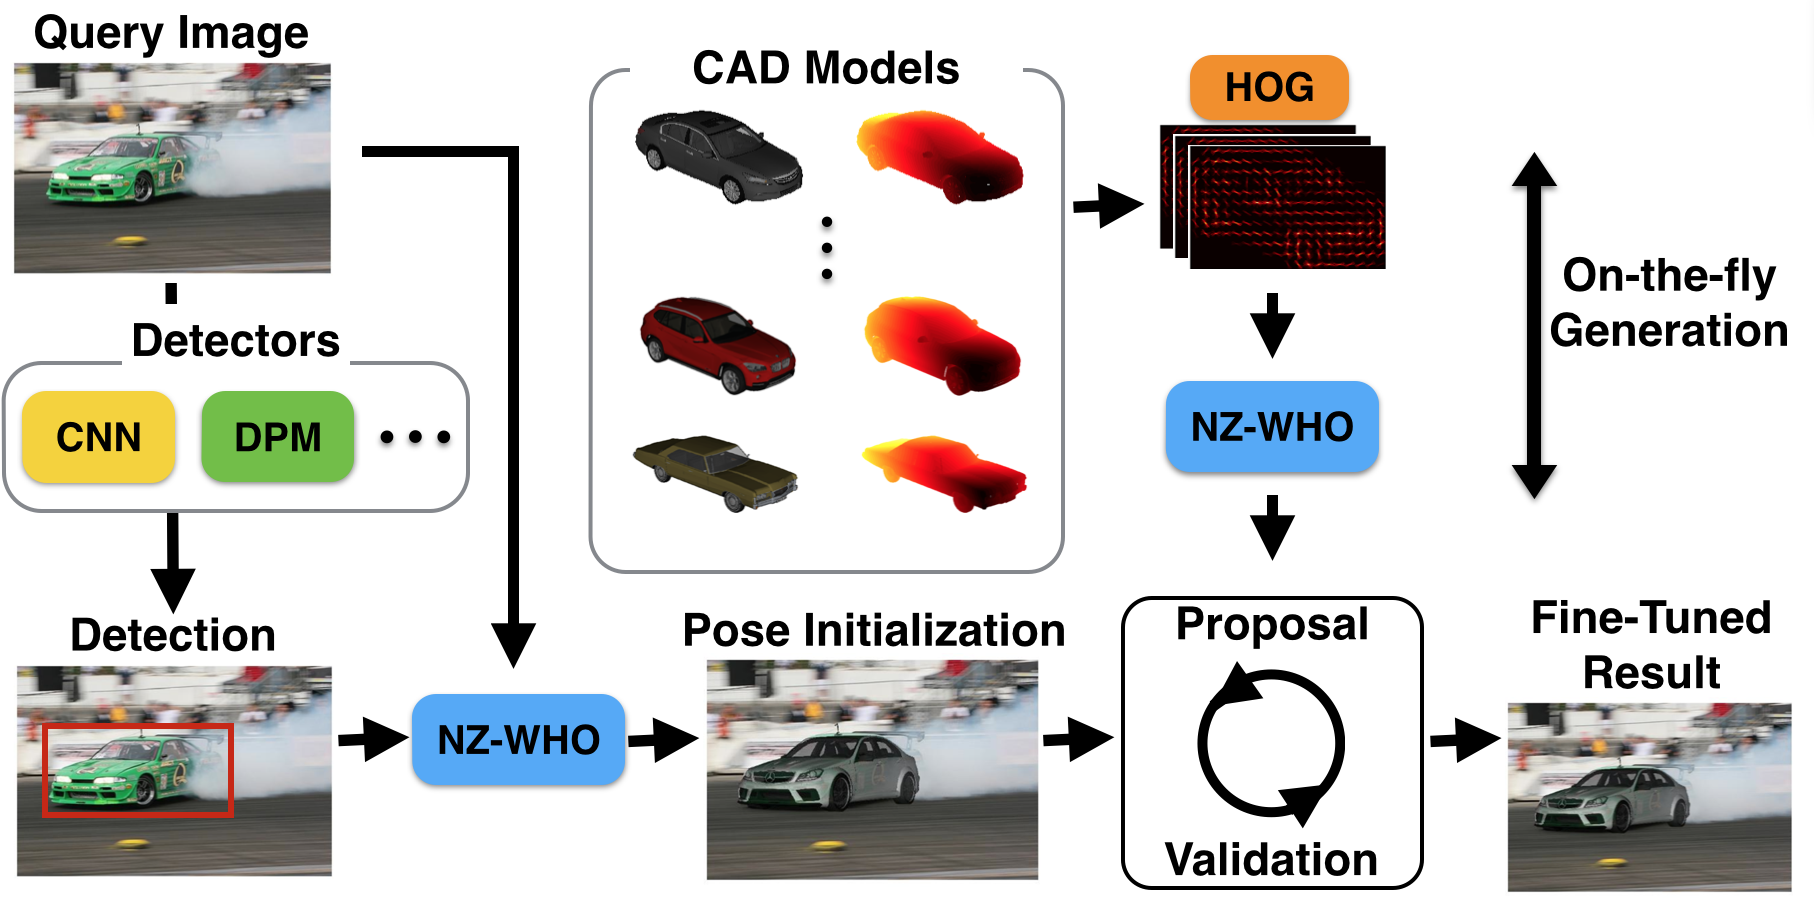
\includegraphics[width=0.95\linewidth]{front} % \\[-5pt]
          \caption{\normalfont Using a database of 3D CAD models, we generate NZ-WHO
            templates which can be used to either detect objects directly or
            enrich the output of an existing detector with high-quality,
            continuous pose and 3D CAD model exemplar.}
          \label{fig:front}
        \end{figure}
        % \vspace{-1.0em}

        % \begin{itemize}
        %   \item Create an ensemble of NZ-WHO templates
        %   \item Initialize viewpoint
        %   \item Propose and validate using Single component Metropolis-Hastings
        %     algorithm
        % \end{itemize}
      \end{block}


    \end{column}%1



    %-----------------------------------------------------
    % Column 2 
    %-----------------------------------------------------
    \begin{column}{0.24\linewidth}


      %-- Block 2-1 --------------------------------------
      \begin{block}{Non-Zero Whitened Histograms of Orientations (NZ-WHO)}
        \vspace{-1.0em}
        \begin{itemize}
          \item CAD rendering introduces textureless background as in
            Fig.~\ref{fig:whocomparison}
          \item The textureless region results in strong negative
            weights Fig.~\ref{fig:whocomparison}.

          \item $\bar{n}$ be the number of non-zero HOG cells, and a matrix
            $S\in \mathcal{R}^{\bar{n}d \times nd}$ be the masking matrix that
            selects non-zero HOG cells.

            % For instance, a template has  $n=3,
            % \bar{n}=2$, and only the second HOG cell has $0$ norm, then

            % \begin{align}
            %     S = \left[ \begin{array}{ccc}
            %         I_d & \mathbf{0} & \mathbf{0}\\
            %         \mathbf{0} & \mathbf{0} & I_d
            %         \end{array} \right]
            % \end{align}

          \item $\bar{x} = S x, \bar{\mu} = S\mu, \bar{\Sigma} = S \Sigma S^T$. 
            \begin{equation}
              \bar{w}=\bar{\Sigma}^{-1}(\bar{x} - \bar{\mu}) \label{eq:nz-who}
            \end{equation}
        \end{itemize}

        \begin{figure}[t]
          \begin{center}
            \small
            \setlength\tabcolsep{3pt}
            \begin{tabular}{|c|c|c|c|c|}
              \hline
              Rendering & WHO$_+$ & WHO$_-$  & NZ-WHO$_+$ & NZ-WHO$_-$ \\
              \hline
              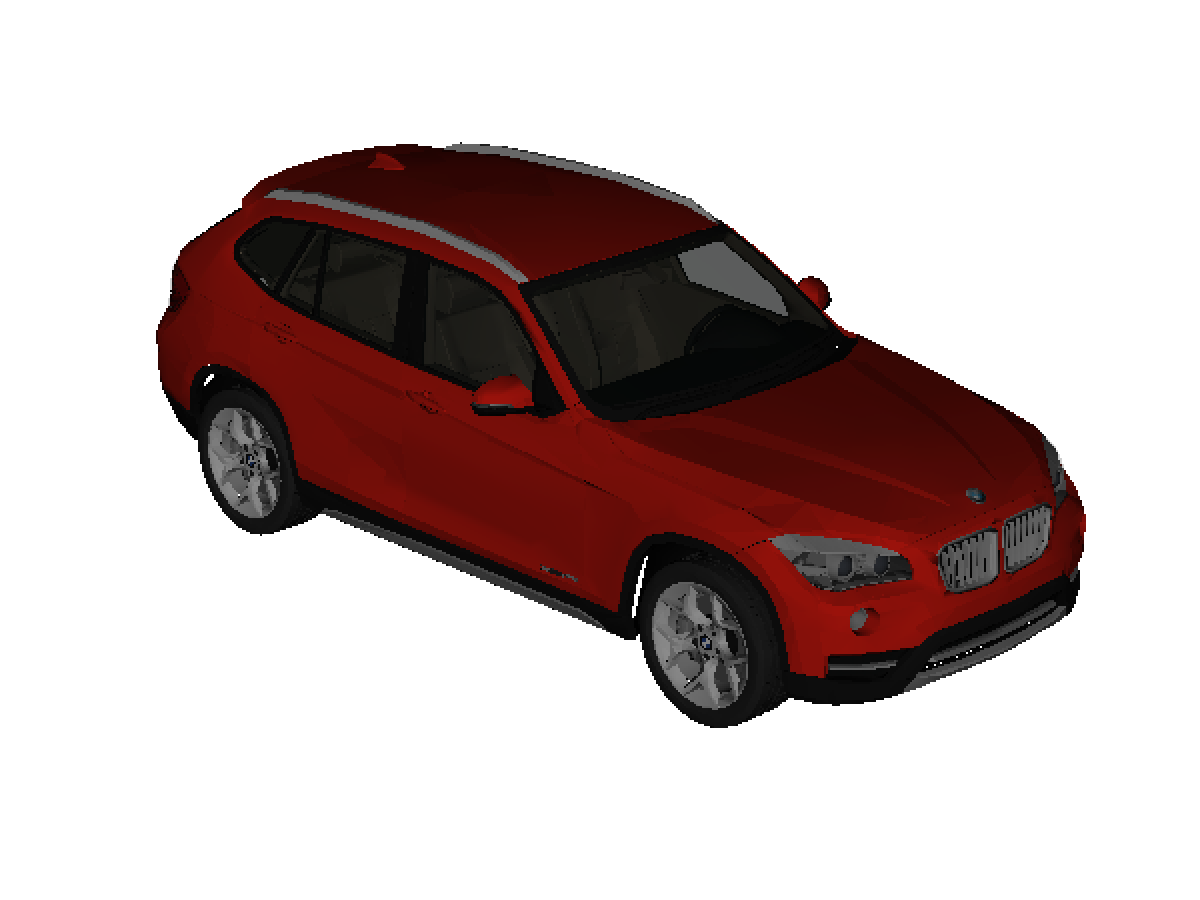
\includegraphics[width=0.16\linewidth]{rendering} &
              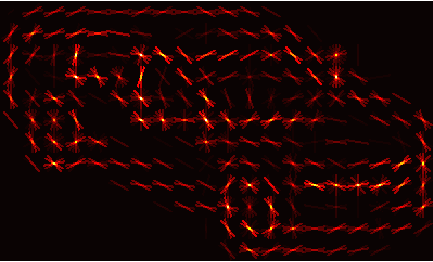
\includegraphics[width=0.18\linewidth]{whiten_all_crop} &
              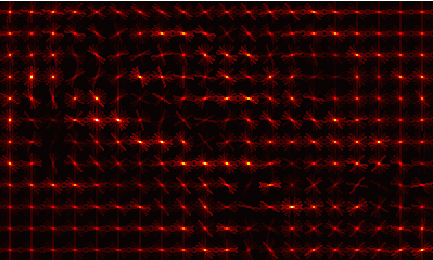
\includegraphics[width=0.18\linewidth]{whiten_all_neg_crop}  &
              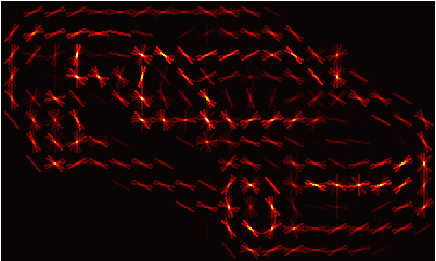
\includegraphics[width=0.18\linewidth]{whiten_non_zero_crop} &
              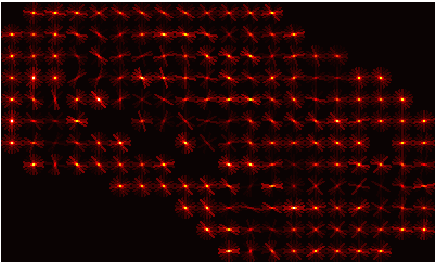
\includegraphics[width=0.18\linewidth]{whiten_non_zero_neg} \\
              \hline
            \end{tabular}
          \end{center}
          \caption{Rendering, WHO, NZ-WHO comparison. Whitening all cells in
            WHO results in strong negative edges on the empty region.}
          \label{fig:whocomparison}
        \end{figure}

        % \begin{figure}[t]
        %   \begin{center}
        %     \setlength\tabcolsep{3pt}
        %     \begin{tabular}{ccc}
        %       HOG & WHO & NZ-WHO \\
        %       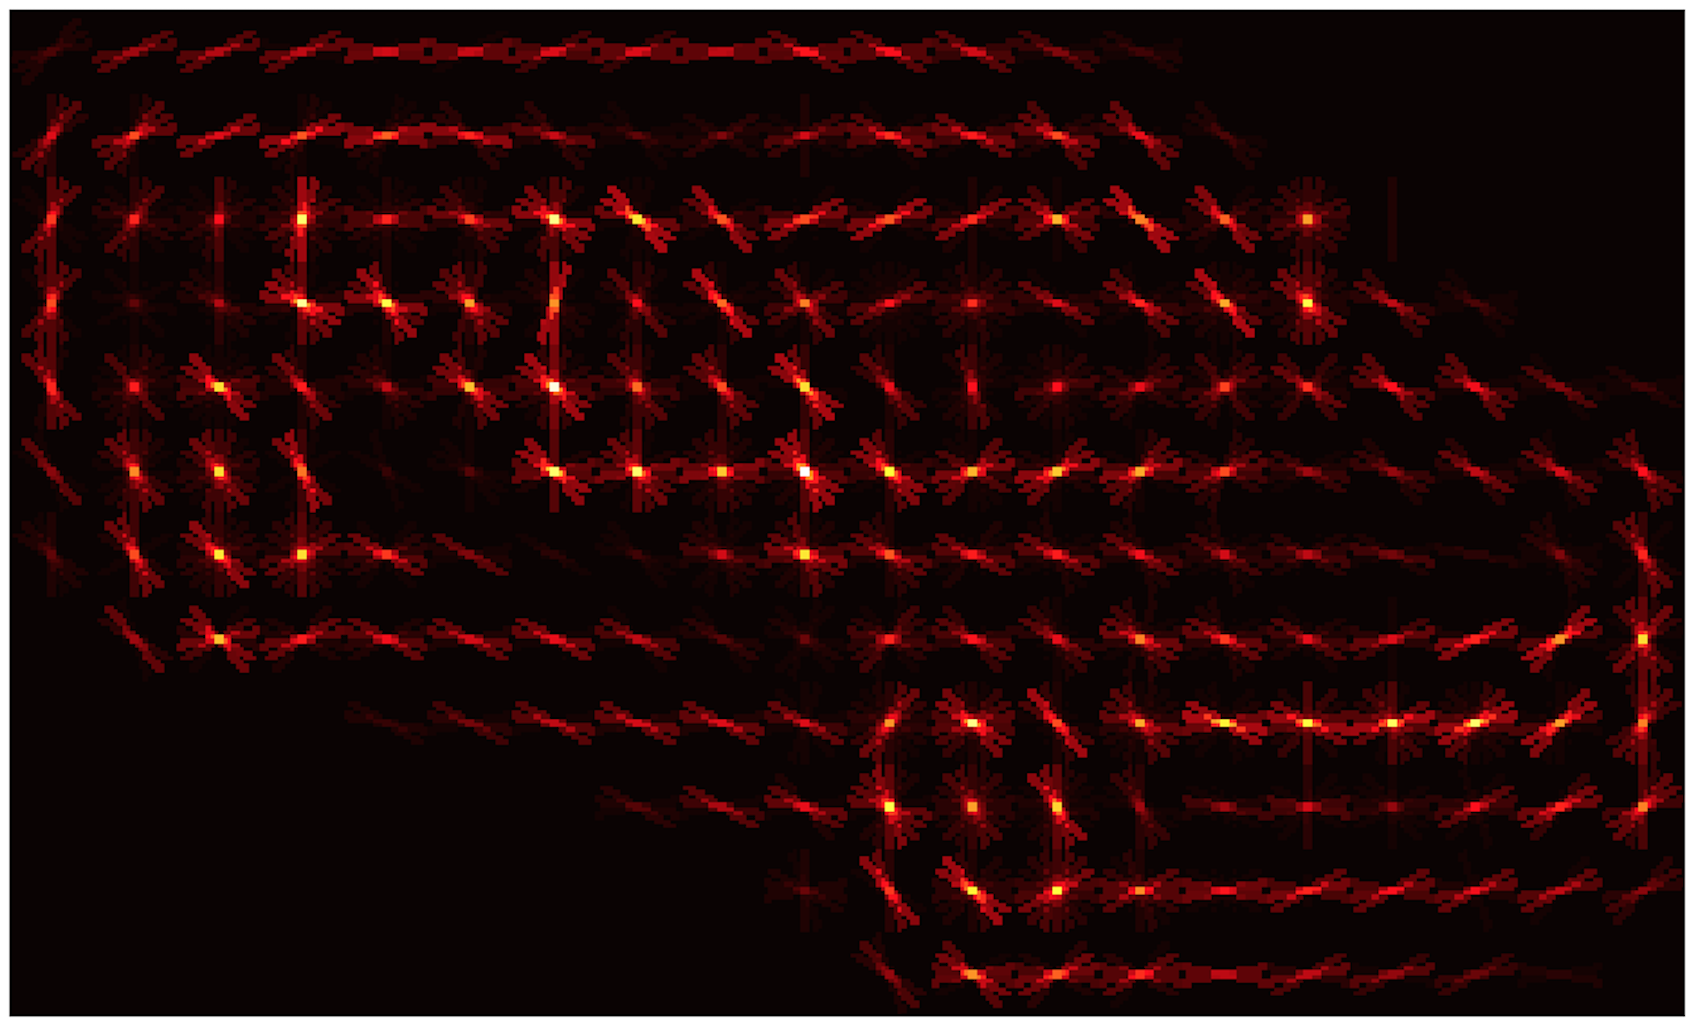
\includegraphics[width=0.2\linewidth]{hog_crop} &
        %       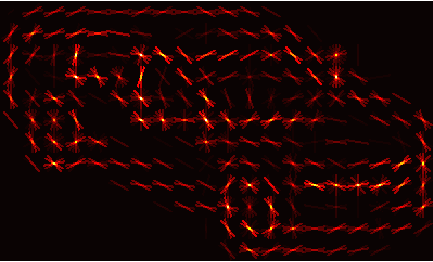
\includegraphics[width=0.2\linewidth]{whiten_all_crop} &
        %       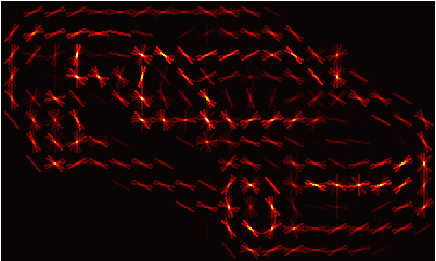
\includegraphics[width=0.2\linewidth]{whiten_non_zero_crop} \\
        %       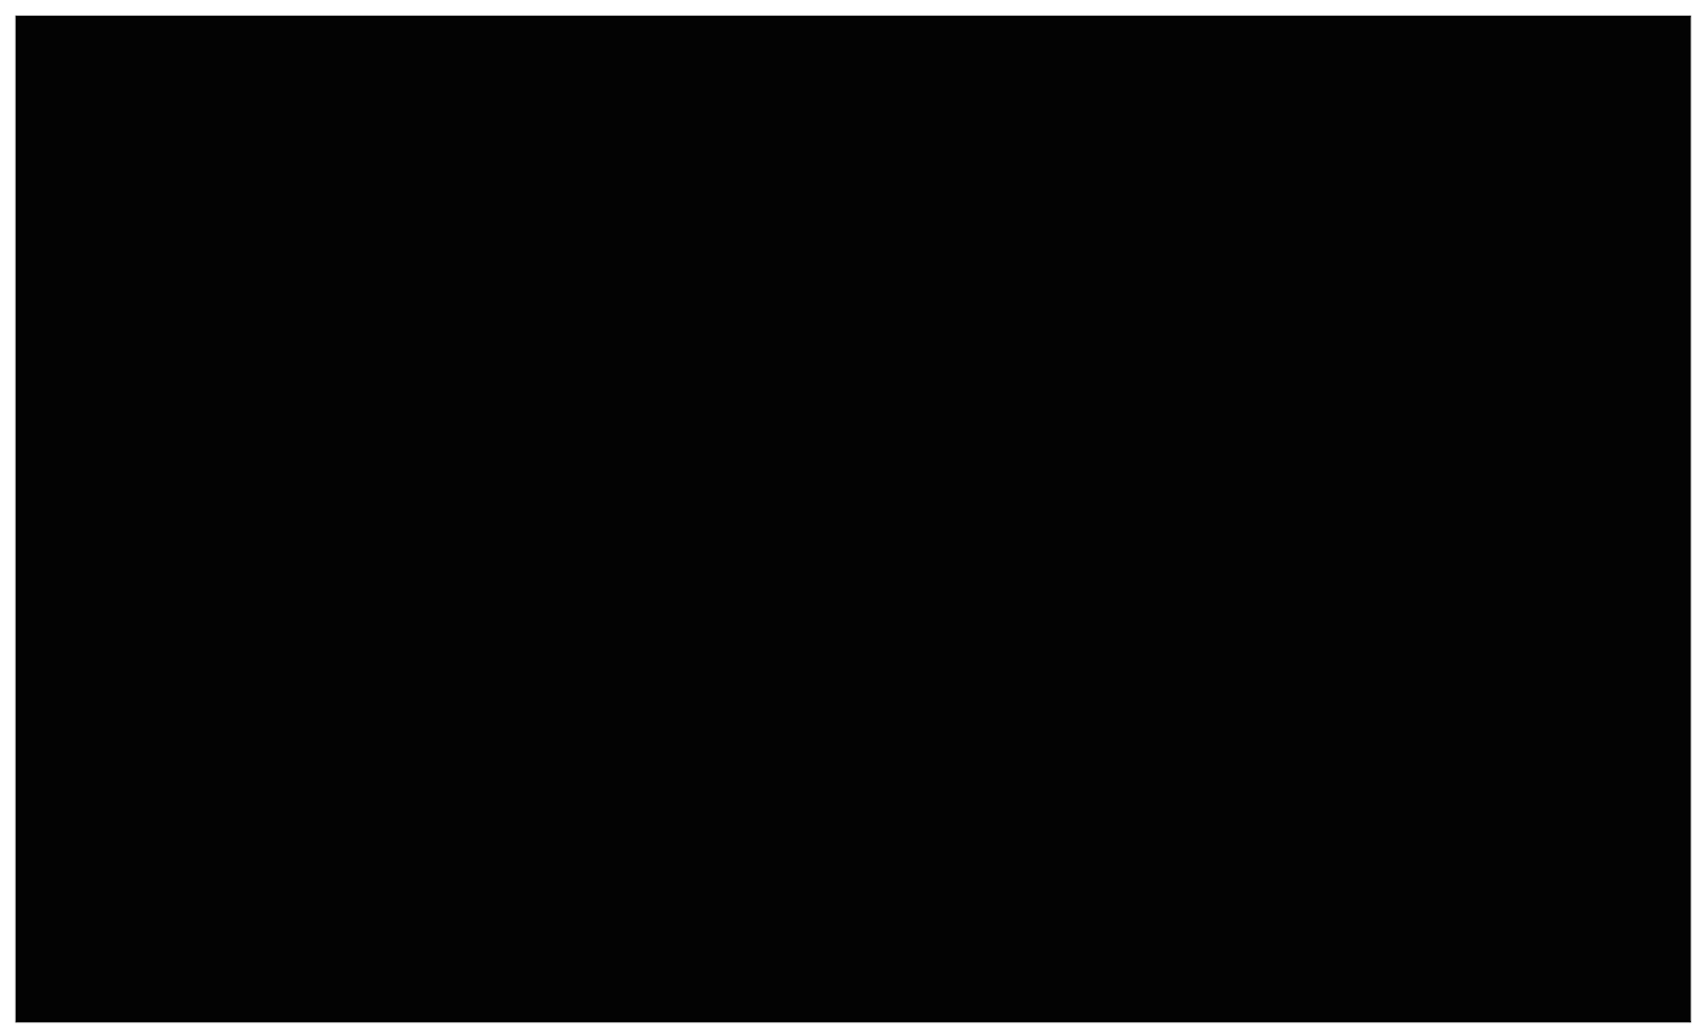
\includegraphics[width=0.2\linewidth]{hog_neg_crop} &
        %       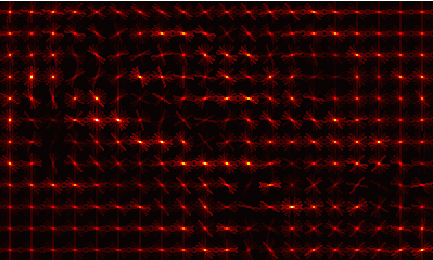
\includegraphics[width=0.2\linewidth]{whiten_all_neg_crop}  &
        %       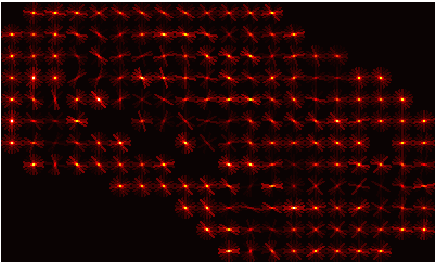
\includegraphics[width=0.2\linewidth]{whiten_non_zero_neg} \\
        %       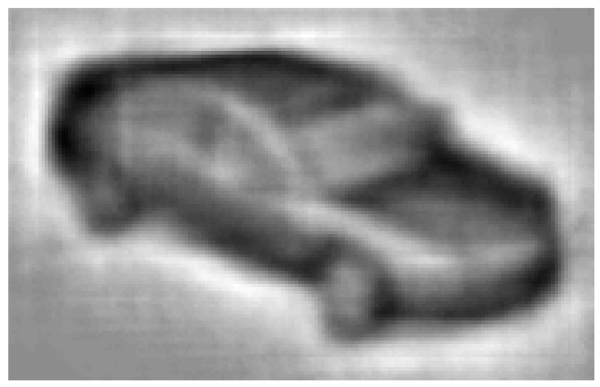
\includegraphics[width=0.2\linewidth]{ihog_hog200_crop.png} &
        %       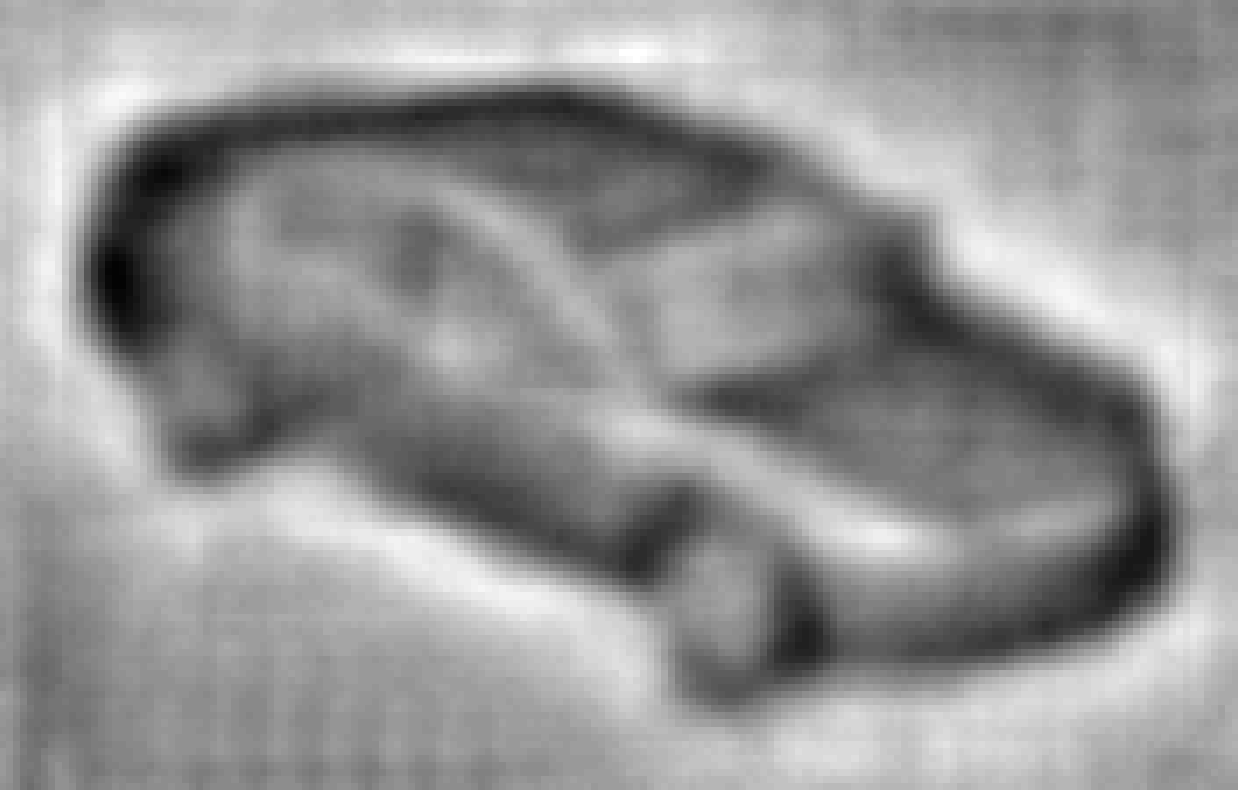
\includegraphics[width=0.2\linewidth]{ihog_whiten_all200_crop.png} &
        %       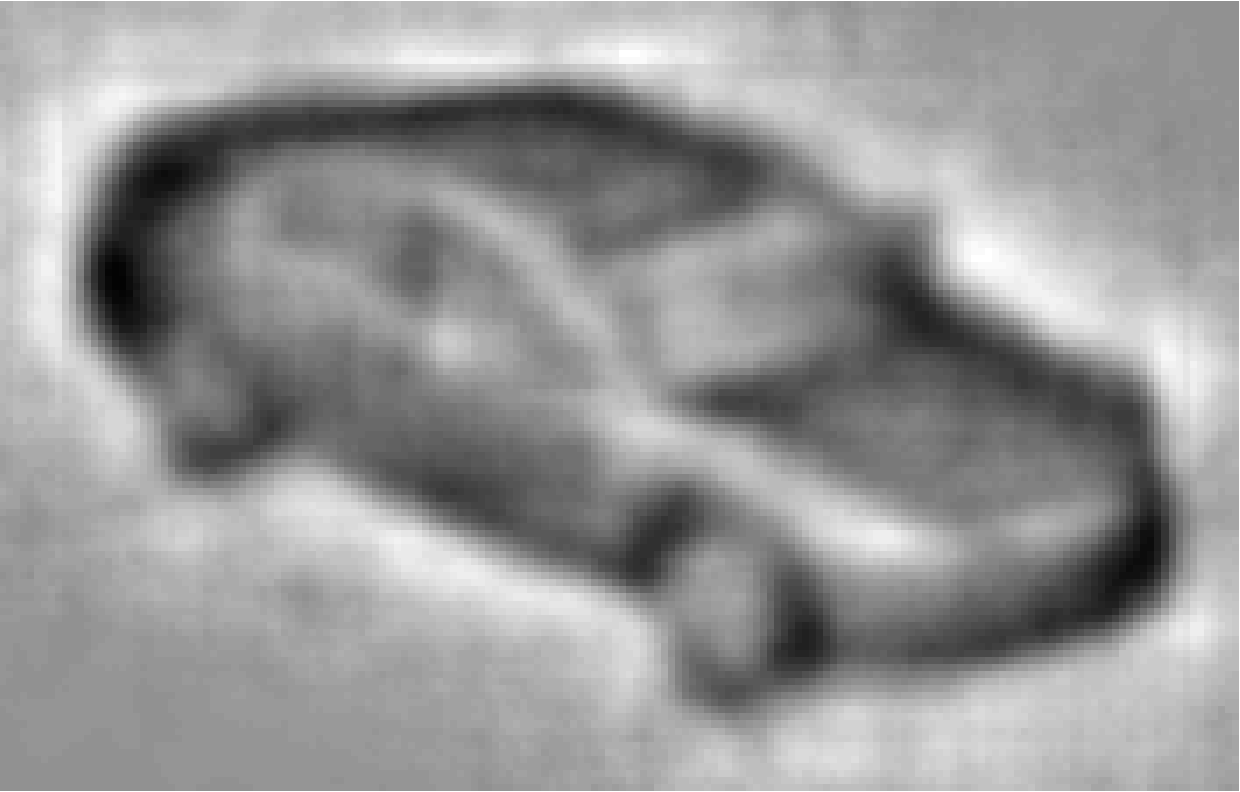
\includegraphics[width=0.2\linewidth]{ihog_whiten_non_zero200_crop.png} \\
        %     \end{tabular}
        %   \end{center}
        %   \caption{Comparison of HOG, WHO and NZ-WHO. Visualization of positive
        %     weights (first row),  visualization of negative weights (second row),
        %     HOGgles (third row). Note that for WHO, whitening all cells results
        %     in strong negative edges on the empty region.}
        %   \label{fig:whocomparison}
        % \end{figure}

        \vspace{-1.0em}
      \end{block}

      %-- Block 2-2 --------------------------------------
      \begin{block}{Speedup using Conjugate Gradient method and FFT-Convolution}
        \vspace{-1.0em}
        \begin{itemize}
          \item Cholesky decomposition with Gaussian Elimination: $O(n^3)$
          \item Conjugate Gradient method: $O(n^2\kappa)$ time
            \begin{itemize}
              \item $\kappa$ condition number of the matrix $\Sigma$
            \end{itemize}

          \begin{figure}[t]
            \begin{center}
            \begin{tabular}{ccc}
              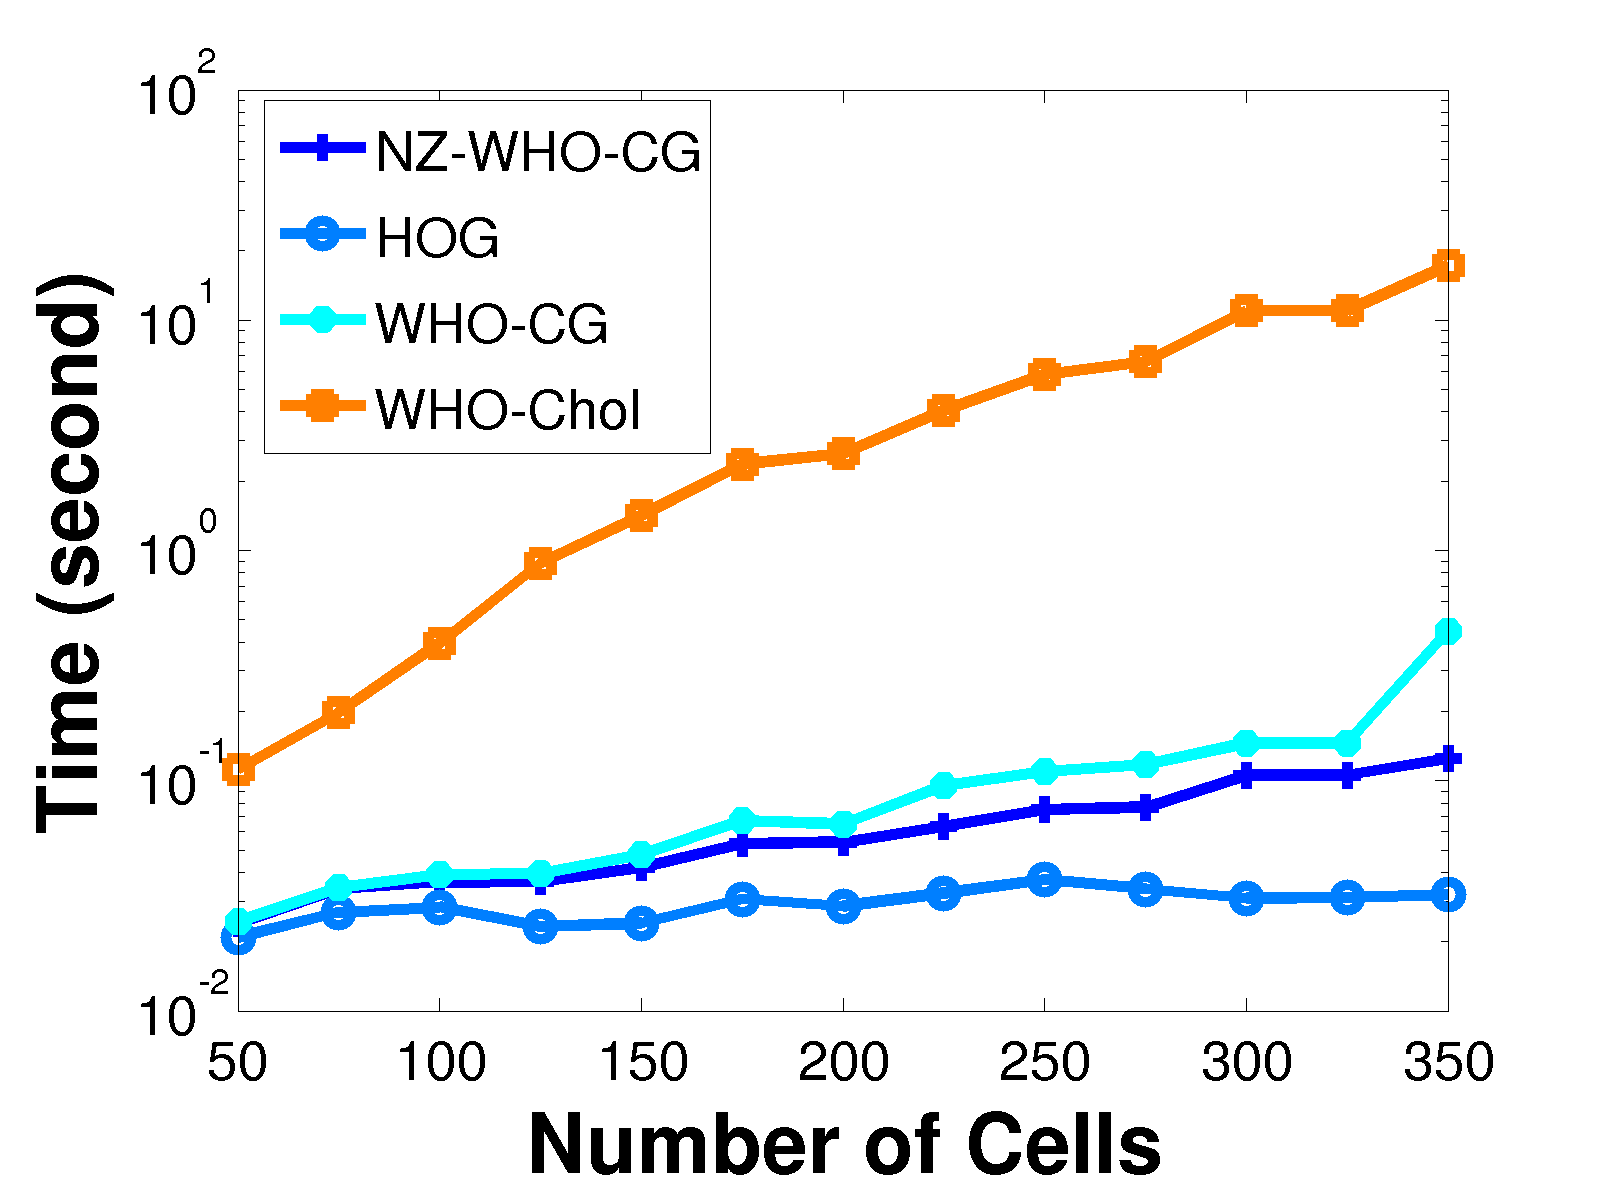
\includegraphics[width=0.3\linewidth]{whotime} &
              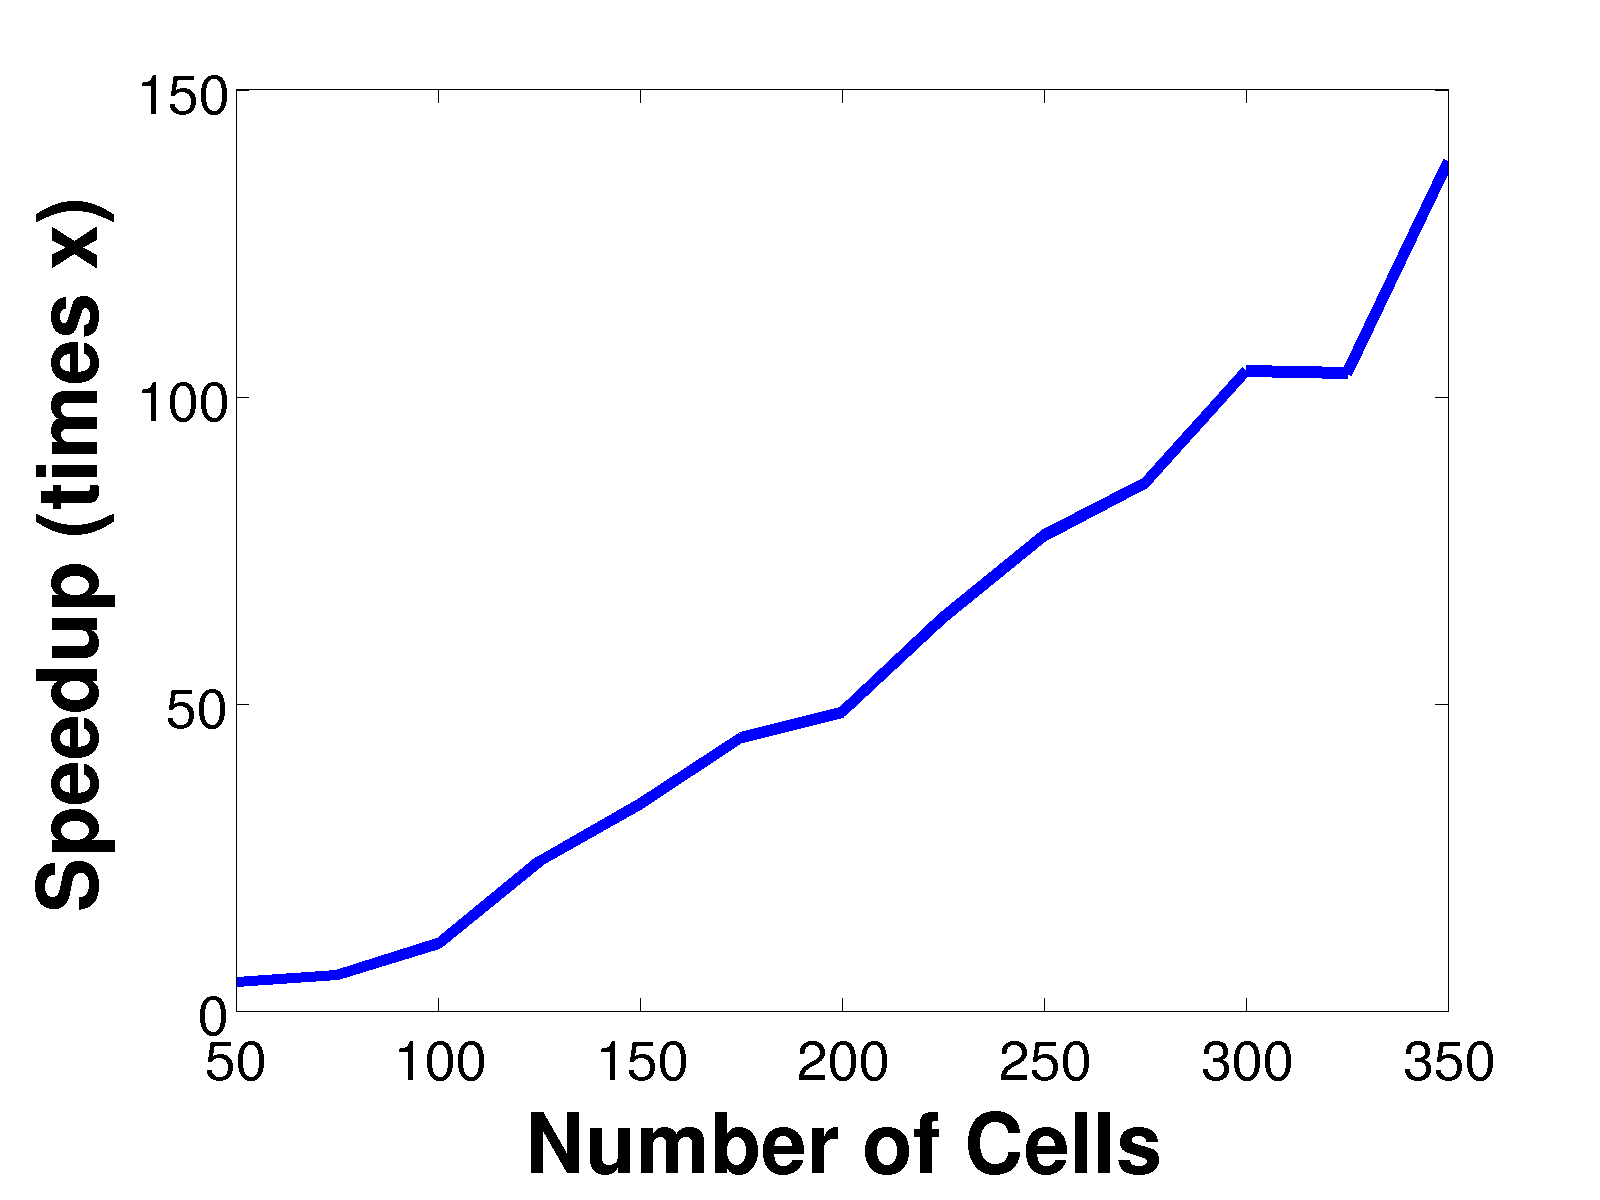
\includegraphics[width=0.3\linewidth]{speedup} &
              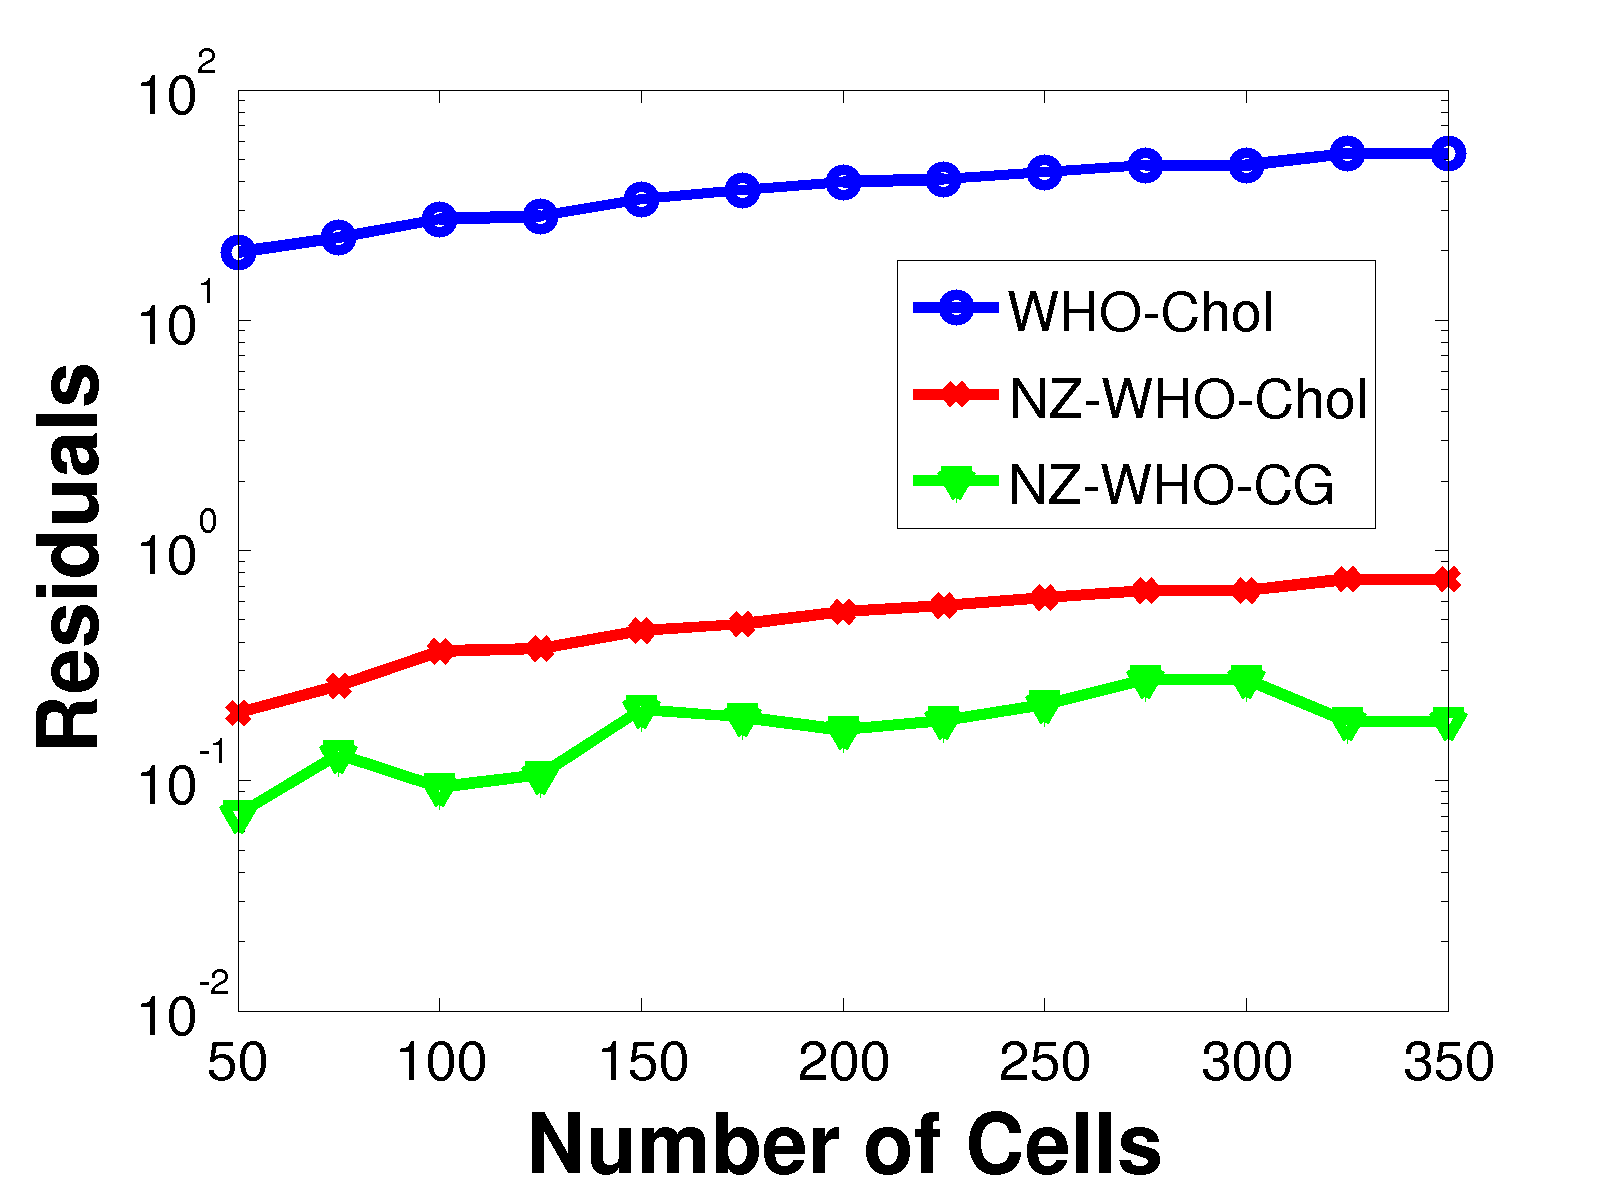
\includegraphics[width=0.3\linewidth]{residual} \\
               (a) & (b) & (c) \\
           \end{tabular}
            \end{center}
            \caption{(a) Runtime analysis of whitening. (b) final speedup
              of NZ-WHO vs. WHO. (c) Residuals of different method}
            \label{fig:whotime}
          \end{figure}
          \item FFT-based Convolution
            \begin{itemize} 
              \item For length $n$ signal and length $m$ filter
              \item Naive convolution takes $O(nm)$ time
              \item FFT-based convolution takes $O\left( (n + m)\log (n+m)
                \right)$ time
              \item High resolution template $\sim 8,000$ dimensional filter
                (template)
            \end{itemize}
        \end{itemize}
      \end{block}


      %-- Block 2-3 --------------------------------------
      \begin{block}{Experiments: NZ-WHO vs WHO}
        \vspace{-1.0em}
        \begin{table}[!htbp]
          \small
          \setlength{\tabcolsep}{1pt}
          \centering
          \begin{tabular}{|c|c|r|c|r|}
            \hline
            Methods (AP/MPPE) & before calib.  & synth. time & after calib. & calib. time \\
            \hline\hline
            HOG      & 72.3 / 65.0          &  31ms  & 60.4 / 50.2           & 8.7 sec \\ 
            WHO  & 82.1 / \textbf{85.4} &  6162ms& 84.4 / 83.0           & 15.4 sec\\
            WHO-CG                 & 81.7 / 84.9          &  104ms & 83.7 / \textbf{87.3}  & 8.3 sec \\
            WHO-CG-Z               & 54.4 / 65.1          &  103ms & \textbf{92.8} / 86.7  & 8.7 sec \\
            % NZC-WHO-Z    & 89.10 /\textbf{78.64} &    & 91.15 / 74.79                  &     \\
            NZ-WHO {\em (ours)} & \textbf{90.0} / 82.8 &   79ms & 90.3 / 86.8           & 8.5 sec \\
            \hline
          \end{tabular}
          \caption{\small Average Precision (AP), Mean Precision in Pose Estimation
            (MPPE) of variants of WHO on 3D Object Classes cars, and their
            corresponding synthesis and calibration time per template.}
          % WHO refers to standard WHO using the
          % method presented in \cite{Hariharan12}, WHO-CG uses iterative
          % Conjugate Gradient method to generate WHO. WHO-CG-Z uses whiten the
          % whole template and zero out textureless region. NZ-WHO-CG is the
          % NZ-WHO which whitens only non-zero cells using iterative Conjugate
          % Gradient method. The time column indicates the time to generate one
          % template. We followed calibration procedure presented in \cite{Aubry14}.}
          \label{tab:who_initializations}
        \end{table}
        \vspace{-1.5em}


      \end{block}
    \end{column}%2



    %-----------------------------------------------------
    % Column 3
    %-----------------------------------------------------
    \begin{column}{0.23\linewidth}


      %-- Block 3-2 --------------------------------------
      \begin{block}{Fine-Tuning via MCMC}
        \begin{itemize}
          \item Continuous parameter $\theta = [v, m, f]$
            \begin{itemize}
              \item $v$ is the 3D rotation of the CAD model
              \item $m$ is the CAD model index
              \item $f$ is the focal length
            \end{itemize}
            \begin{align}
                P(\theta| \mathcal{I}) & \sim e^{ \max_{s} w(\theta) \ast
                  \mathcal{T}_s(\mathcal{I})},
            \end{align}
            \begin{itemize}
              \item $\max_{s} w(\theta) \ast T_s(\mathcal{I})$ is the maximum
                convolution score of NZ-WHO template with image features for
                all scale $s$
            \end{itemize}
          \item Approximate the MAP solution
            \begin{itemize}
              \item Draw samples using Single Component Metropolis-Hastings
            \end{itemize}
          \item Proposal distributions for each component are
            \begin{align}
                g(\theta \rightarrow \theta(v_i^+)) & \sim
                \mathcal{N}(\theta_{v_i},\sigma_v) \quad \mbox{ for }\; i \in \{1,2,3\}\\
                g(\theta \rightarrow \theta(f^+)) & \sim \mathcal{N}(\theta_{f}, \sigma_f)\\
                g(\theta \rightarrow \theta(m^+)) & \sim (1-c) \delta(\theta_m) +
                c\,\textrm{Unif}(1,M)
            \end{align}
        \end{itemize}
      \end{block}


      %-- Block 3-3 --------------------------------------
      \begin{block}{Experiments}
        \begin{figure}
          \begin{center}
          \setlength\tabcolsep{0pt}
          \begin{tabular}{|c|c|}
            \hline
            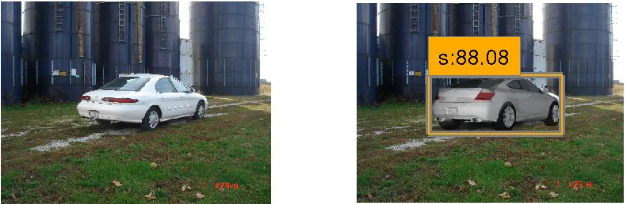
\includegraphics[width=0.40\linewidth]{supp/car32.png} &
            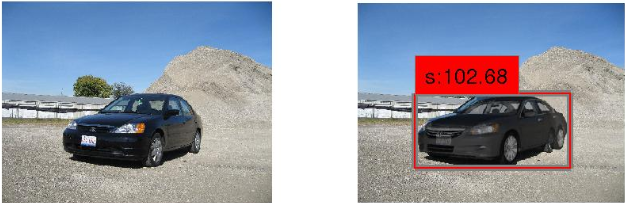
\includegraphics[width=0.40\linewidth]{supp/car26.png} \\
            % 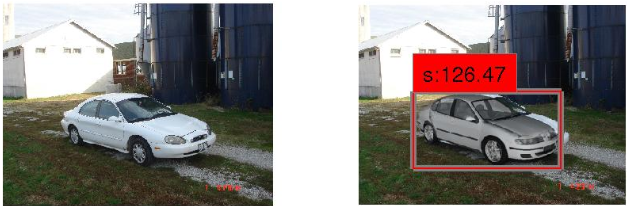
\includegraphics[width=0.40\linewidth]{supp/car20.png} & 
            % 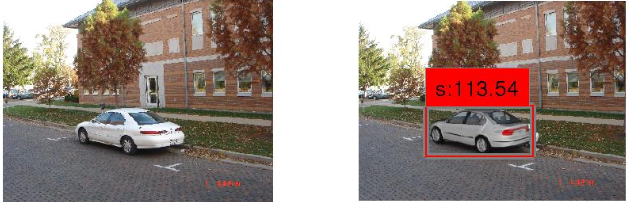
\includegraphics[width=0.40\linewidth]{supp/car31.png} \\
            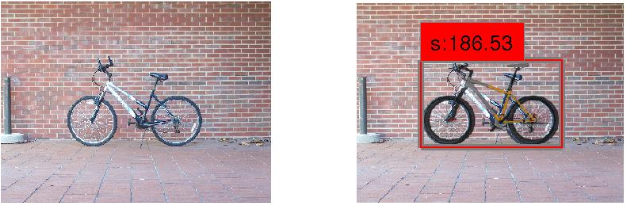
\includegraphics[width=0.40\linewidth]{supp/bicycle16.png} &
            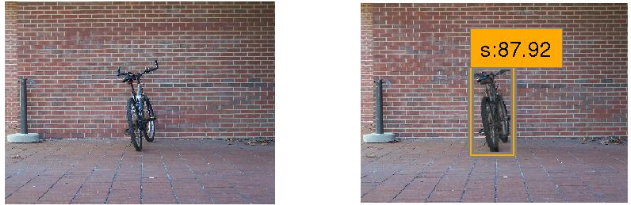
\includegraphics[width=0.40\linewidth]{supp/bicycle12.png} \\
            % 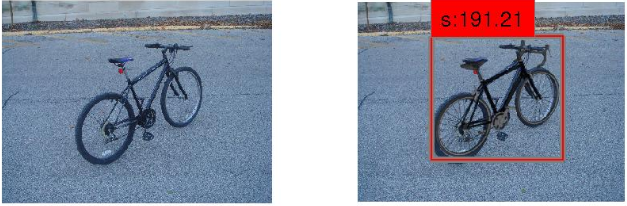
\includegraphics[width=0.40\linewidth]{supp/bicycle15.png} &
            % 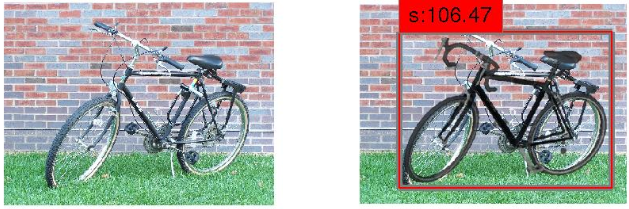
\includegraphics[width=0.40\linewidth]{supp/bicycle10.png} \\
            \hline
          %  (c) & (d) \\[0pt]
          \end{tabular}
          \end{center}
          \caption{\small Detection results on 3D Object Classes. Original image
            (left) and detection result overlaid on top (right).}
          \label{fig:3dobject_vis}
        \end{figure}
        \vspace{-1.0em}
\begin{table*}[t]
    \scriptsize
  \begin{center}
    \begin{tabular}{|c||c||c||c|c||c|c|}
    \hline
    AP/AVP              & V-DPM \cite{Xiang14} & DPM-VOC+VP \cite{Pepik12}  & \cite{Pepik12} + Ours (discrete) & \cite{Pepik12} + Ours (full) & R-CNN + Ours (discrete) & R-CNN + Ours (full)\\
    \hline\hline
%    aeroplane-4v        & 40.0 / 34.6         & 41.5 / 37.4             & 41.1 / 32.7       & 41.1 / 30.5        & 67.8 / \textbf{41.3}         & 67.8 / 40.8 \\ \hline
%    aeroplane-8v        & 39.8 / 23.4         & 40.5 / 28.6             & 41.1 / 26.8       & 41.1 / 24.2        & 67.8 / 26.8         & 67.8 / \textbf{27.4} \\ \hline
%    aeroplane-16v       & 43.6 / 15.4         & 38.0 / 15.9             & 41.1 / 17.7       & 41.1 / 16.3        & 67.8 / 21.2         & 67.8 / \textbf{21.5} \\ \hline
%    aeroplane-24v       & 42.2 / 8.0          & 36.0 /  9.7             & 41.1 / 10.9       & 41.1 / 10.2        & 67.8 / 15.6         & 67.8 / \textbf{15.7} \\ \hline
%    \hline
    car-4v              & 37.2 / 20.2         & 45.6 / 36.9             & 47.6 / 42.7       & 47.6 / \textbf{42.7}        & 49.6 / 41.5         & 49.6 / 41.5\\ \hline
    car-8v              & 37.3 / 23.5         & 47.6 / 36.6             & 47.6 / \textbf{39.8}       & 47.6 / 39.5        & 49.6 / 38.0         & 49.6 / 39.0\\ \hline
    car-16v             & 36.6 / 18.1         & 46.0 / 29.6             & 47.6 / 32.7       & 47.6 / 33.0        & 49.6 / 34.0         & 49.6 / \textbf{34.3}\\ \hline
    car-24v             & 36.3 / 13.7         & 42.1 / 24.6             & 47.6 / 27.4       & 47.6 / 27.4        & 49.6 / 27.0         & 49.6 / \textbf{27.6}\\ \hline
    \hline
%    chair-4v            & 11.1 / 6.8          & 8.7  / 6.1              &  11.4 / 7.1       & 11.4 / 6.7         & 25.2 / 10.6         & 25.2 / \textbf{10.7} \\ \hline
%    chair-8v            & 11.4 / 5.9          & 11.3 / 9.4              &  11.4 / 6.6       & 11.4 / 6.6         & 25.2 / \textbf{9.4}          & 25.2 / 9.3 \\ \hline
%    chair-16v           & 12.8 / 6.0          & 10.2 / 6.1              &  11.4 / 4.7       & 11.4 / 4.7         & 25.2 / \textbf{6.7}          & 25.2 / 6.7 \\ \hline
%    chair-24v           & 12.6 / 4.4          & 8.0  / 4.2              &  11.4 / 3.1       & 11.4 / 3.4         & 25.2 / 4.6          & 25.2 / \textbf{5.4} \\ \hline
%    \hline
    bicycle-4v          & 45.2 / 41.7         & 46.9 / 43.9             & 48.1 / 47.6       & 48.1 / 46.6        & 61.7 / 56.5         & 61.7 / \textbf{56.7}\\ \hline
    bicycle-8v          & 47.3 / 36.7         & 48.1 / 40.3             & 48.1 / 40.6       & 48.1 / 40.6        & 61.7 / 48.9         & 61.7 / \textbf{49.2}\\ \hline
    bicycle-16v         & 46.5 / 18.4         & 45.6 / 22.9             & 48.1 / 26.2       & 48.1 / 27.3        & 61.7 / 34.7         & 61.7 / \textbf{35.8}\\ \hline
    bicycle-24v         & 44.4 / 14.3         & 45.9 / 16.7             & 48.1 / 21.5       & 48.1 / 20.9        & 61.7 / \textbf{27.0}         & 61.7 / 23.9\\ \hline
    \end{tabular}
  \end{center}
\caption{Average Precision (AP) and Average Viewpoint Precision (AVP) on
  PASCAL3D+~\cite{Xiang14}. For combined methods (* + Ours), we use
  bounding boxes from * and augment viewpoint using our method.}
  % R-CNN
  % and run our method to produce 2D-3D matching. If our method fails to
  % give viewpoint, it predicts the viewpoint to be 0. Note that our
  % method gives high quality metadata such as continuous 3D viewpoint,
  % CAD model (rendering depth) and fine-grained category, whereas
  % base-line methods gives 1D discrete azimuths. Our R-CNN was not an
  % optimized version so the detection AP is lower than the
  % state-of-the-art R-CNN performance}
\label{tab:pascal12}
\end{table*}


        \begin{table}
          \begin{center}
            \begin{tabular}{|c|c|c|c|}
            \hline
            AP/MPPE& Ours & ALM & DPM-VOC+VP \\
            \hline\hline
            car     & \textbf{99.8} / 91.7 & 98.4 / 93.4 & \textbf{99.8} / \textbf{97.5} \\ 
            bicycle & 93.0 / 90.9          & 93.0 / 91.4 & \textbf{98.8} / \textbf{97.5} \\
            \hline
            \end{tabular}
          \end{center}
          \caption{\small Average Precision (AP) and Mean Precision in Pose
            Estimation (MPPE) on 3D Object Classes cars.}% Our method produces high quality 2D-3D matching yet performs on par with state-of-the art detectors.}
          \label{tab:3dobject}
        \end{table}
        \vspace{-1.0em}

        \begin{figure}
          \setlength\tabcolsep{1pt}
          \centering
          \begin{tabular}{c}
          %  \hline
          %  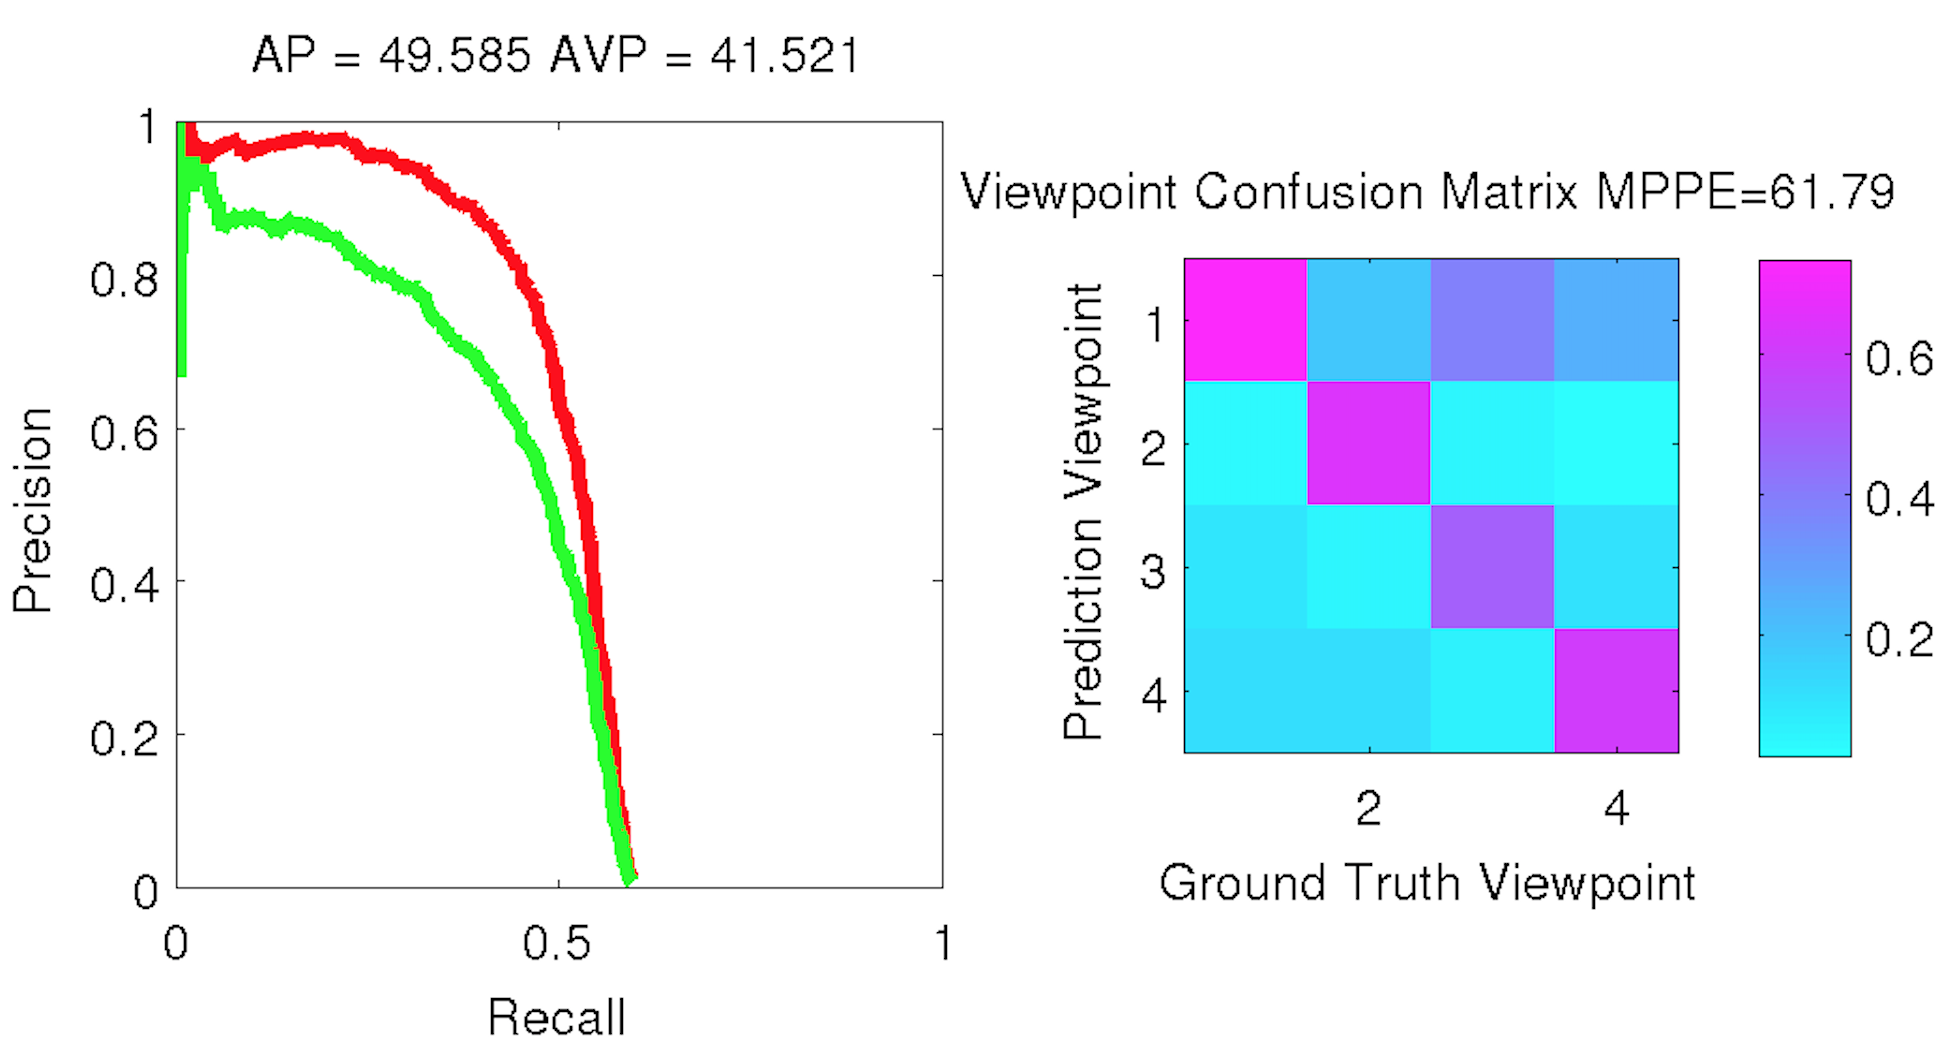
\includegraphics[width=0.49\linewidth]{car_cnn4_crop.png}    
          %  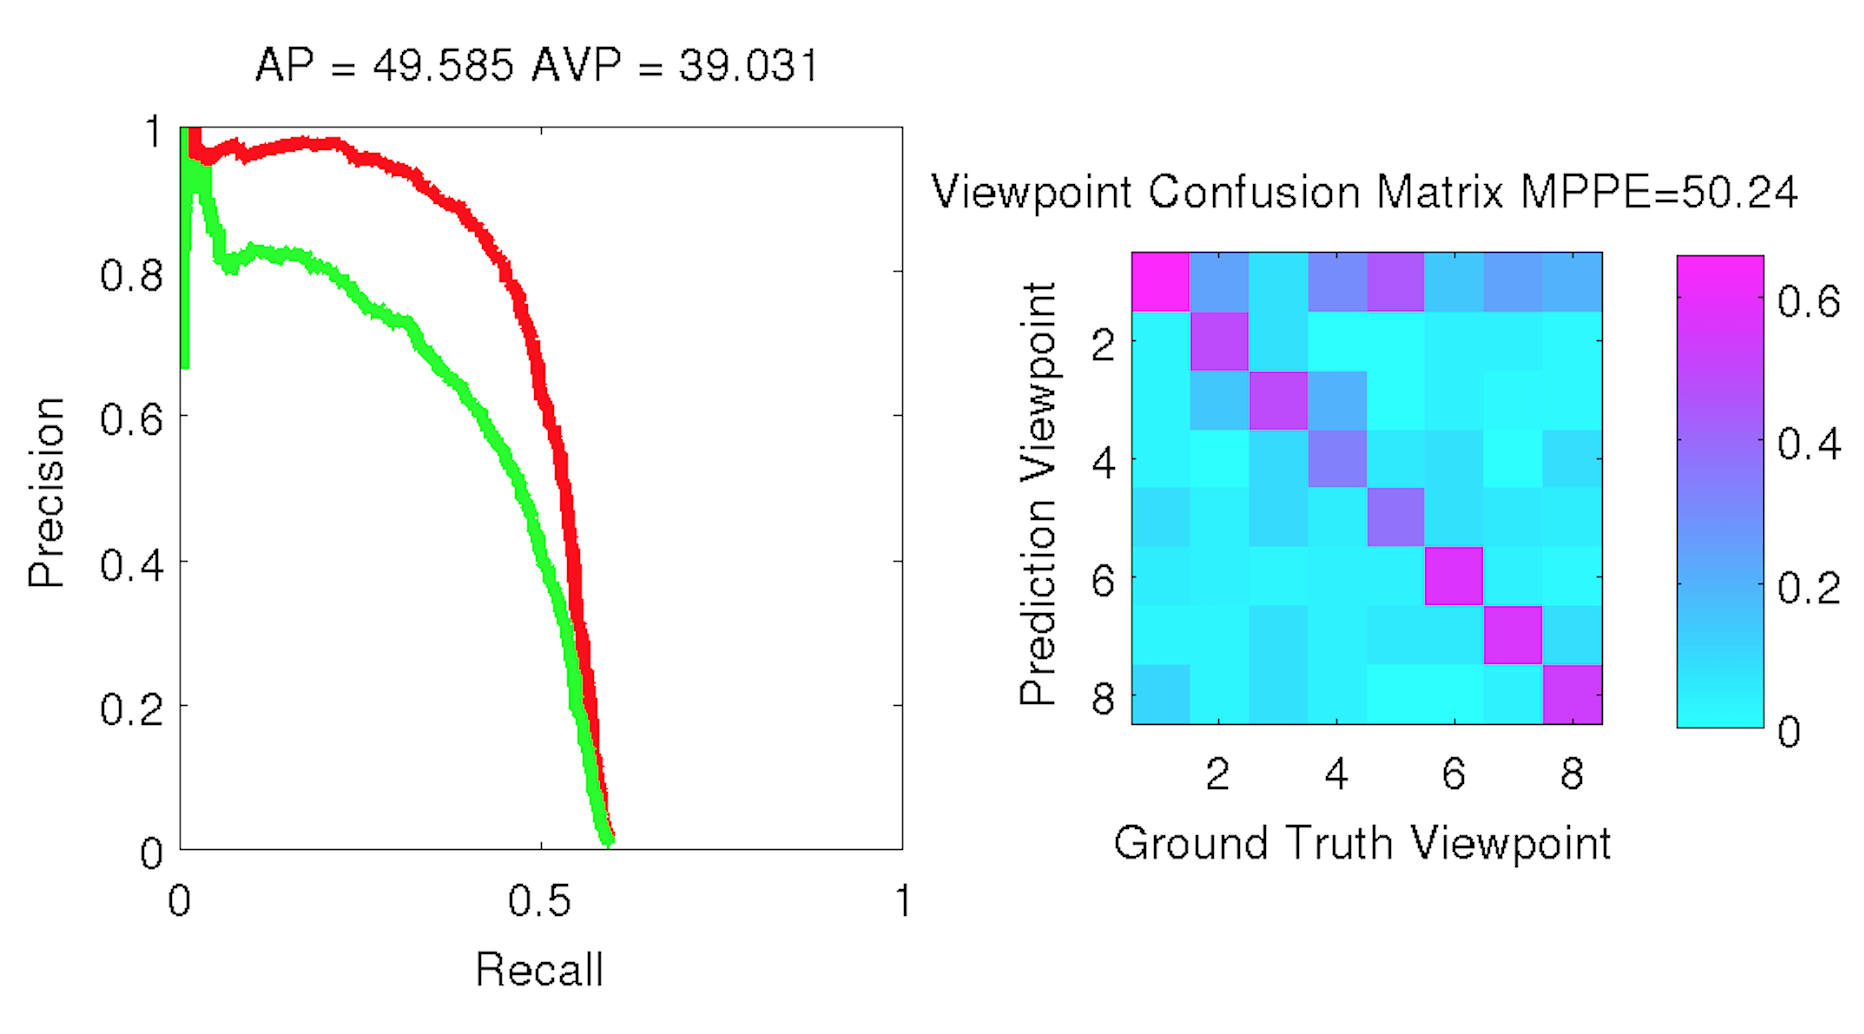
\includegraphics[width=0.49\linewidth]{car_cnn8_crop.png} \\   
          %  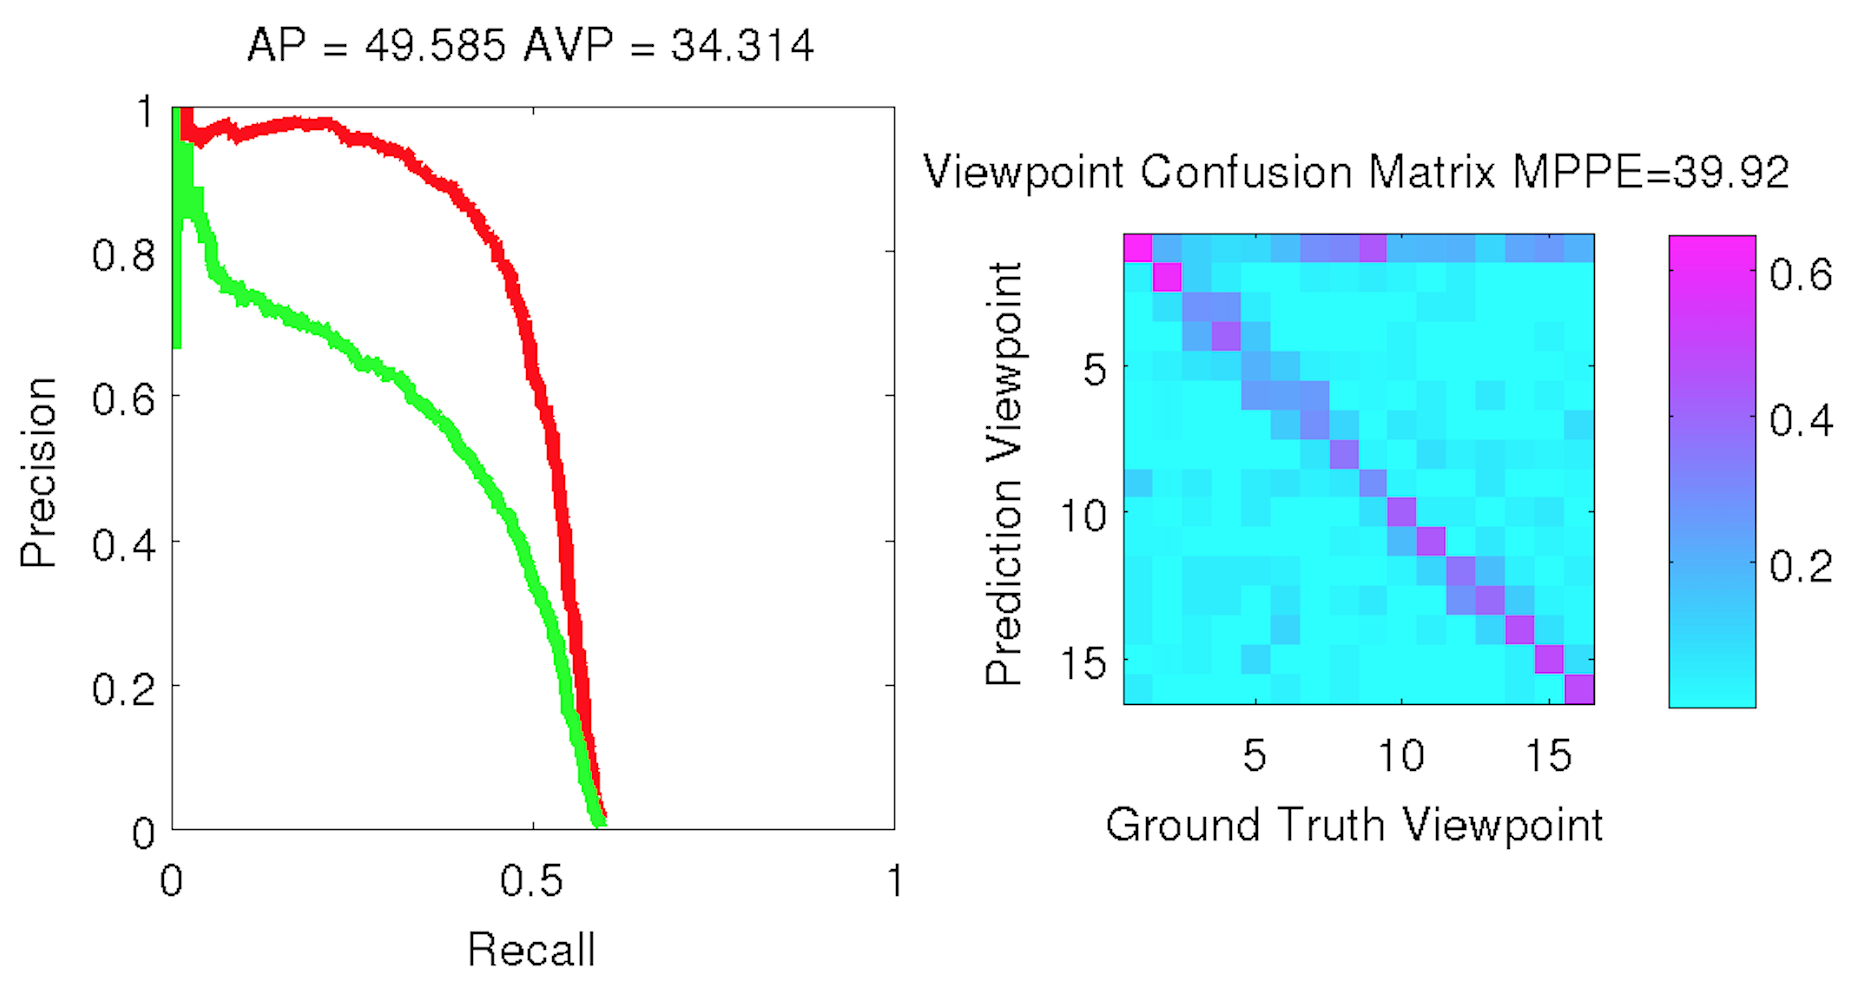
\includegraphics[width=0.49\linewidth]{car_cnn16_crop.png} &   
            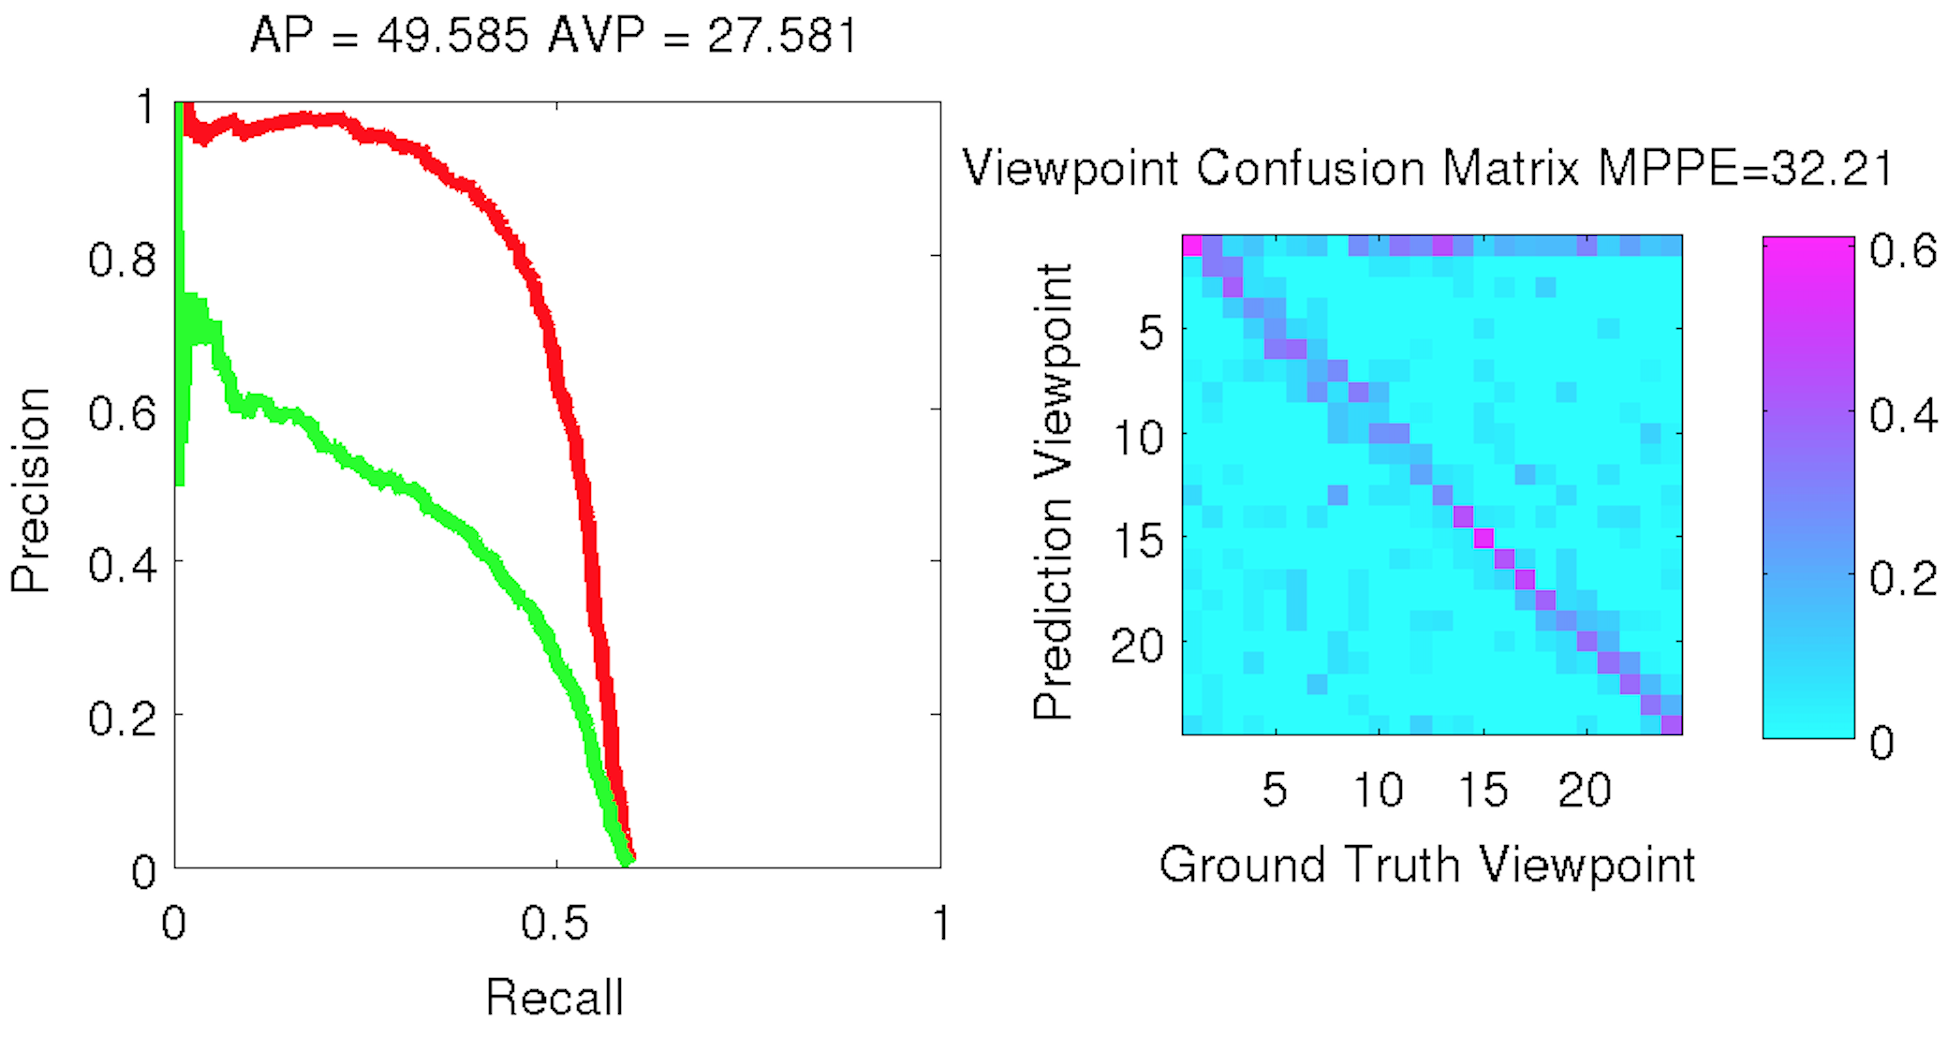
\includegraphics[width=0.6\linewidth]{car_cnn24_crop.png} \\   
          %  \hline
          \end{tabular}
          \caption{\small Average Precision (AP)(red) and Average Viewpoint Precision (AVP)(green)
            and viewpoint confusion table on PASCAL 12 car validation set using
            R-CNN + Ours (full) for 24 views. All four viewpoint discretizations are available on the supplementary paper.}
           % Since our method only augment the object detection,
           %  the AP remains the same for all cases. As we increase the viewpoint
           %  estimation, the AVP decreases. Note that since we estimate null
           %  viewpoint if our method fails to find match, there are more 0
           %  viewpoint predictions (top row of confusion matrices) }
          \label{fig:car_cnn_ap}
        \end{figure}
        \vspace{-1.0em}
      \end{block}
    \end{column}%3


    %-----------------------------------------------------
    % Column 4
    %-----------------------------------------------------       
    \begin{column}{0.23\linewidth}
    %-- Block 3-1
      \begin{block}{Experiments}

        \begin{figure}
        \setlength\tabcolsep{1pt}
        \centering
        \begin{tabular}{|c|c|c|c|c|}
          \hline
          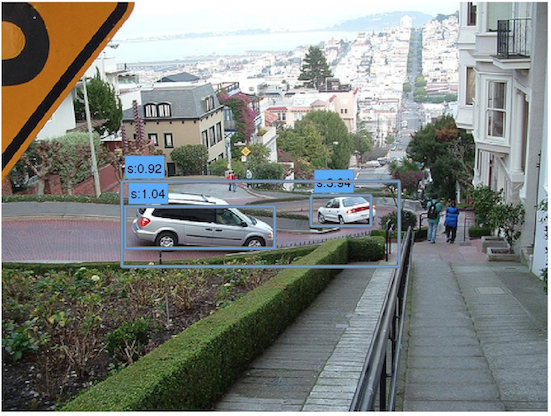
\includegraphics[width=0.24\textwidth]{car_cnn/1a.png} &   
          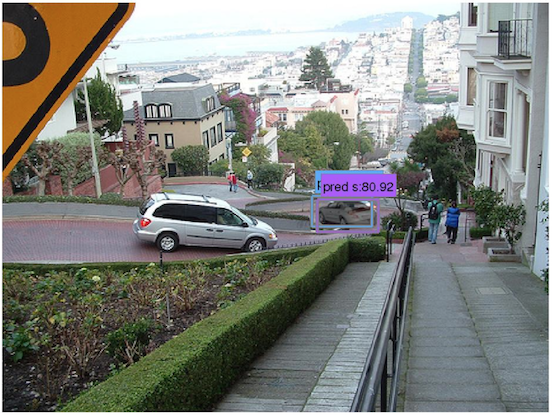
\includegraphics[width=0.24\textwidth]{car_cnn/1b.png} &   
          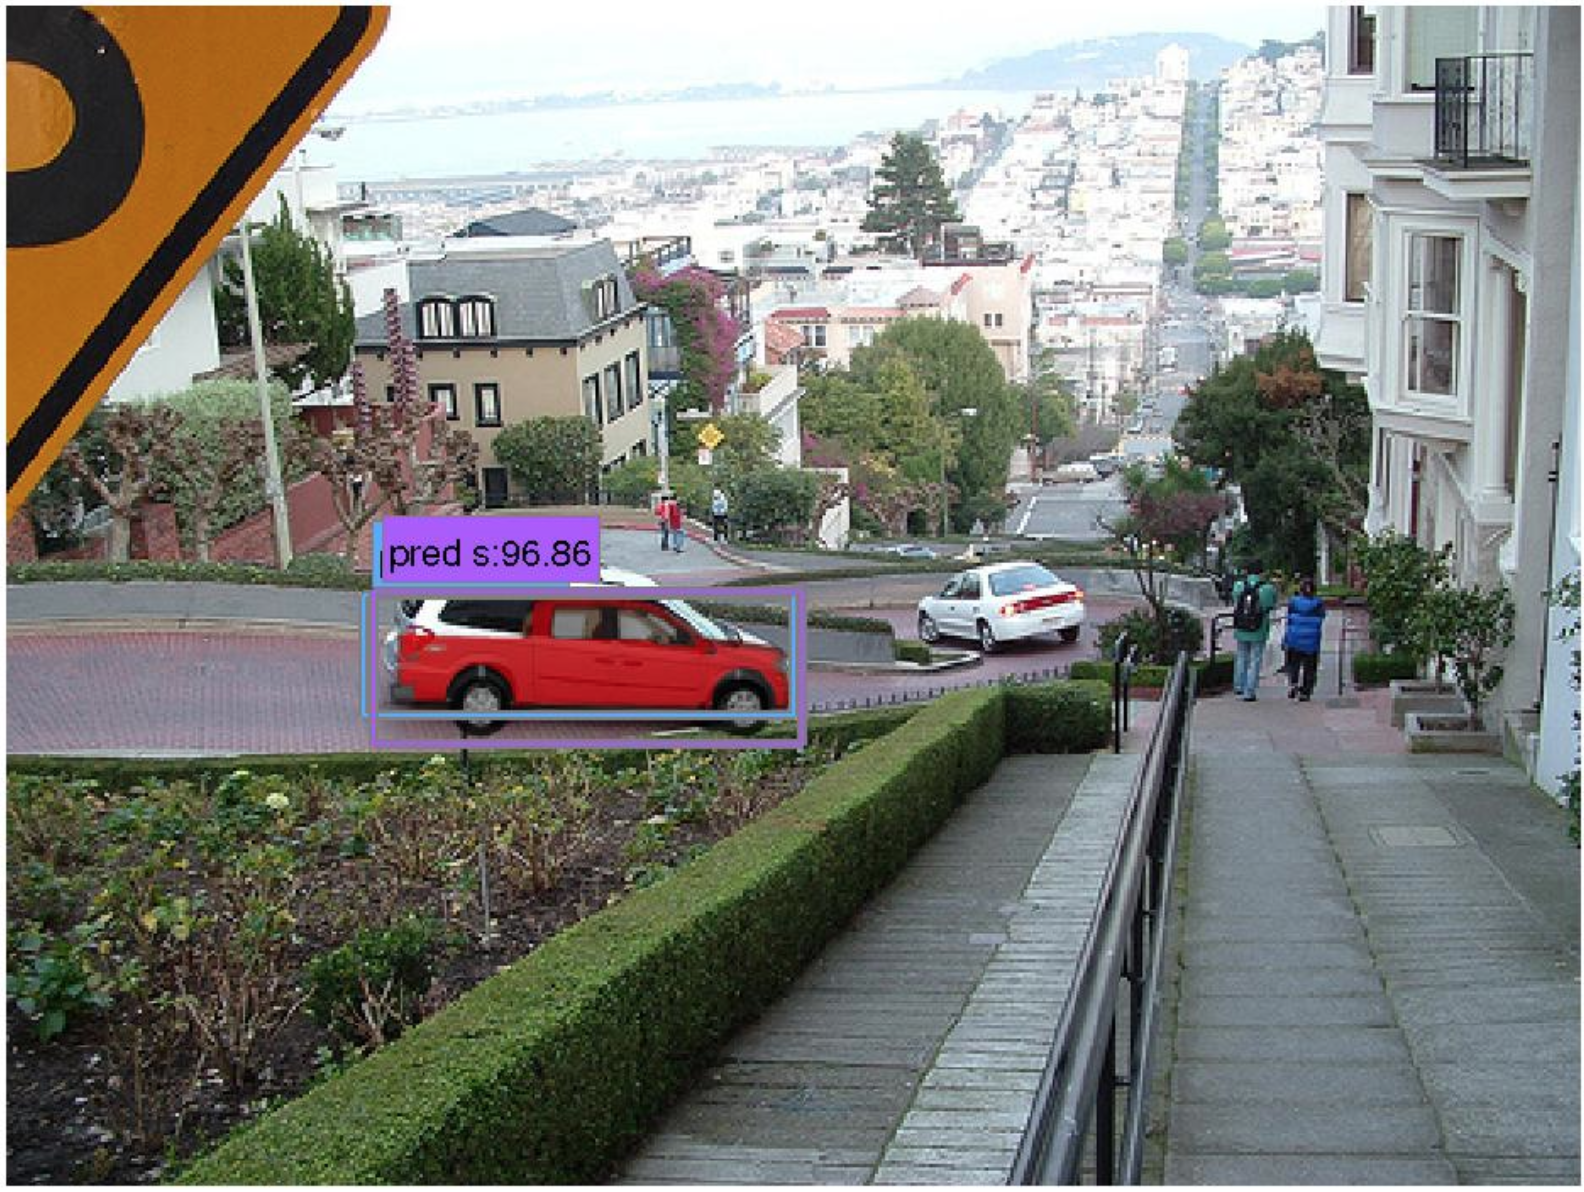
\includegraphics[width=0.24\textwidth]{car_cnn/1c.png} &   
          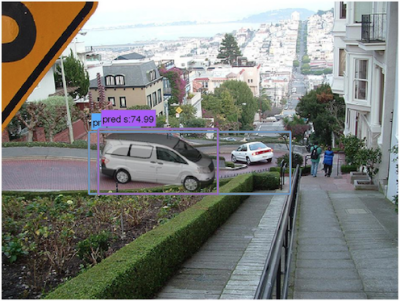
\includegraphics[width=0.24\textwidth]{car_cnn/1d.png}  \\  
          \hline
          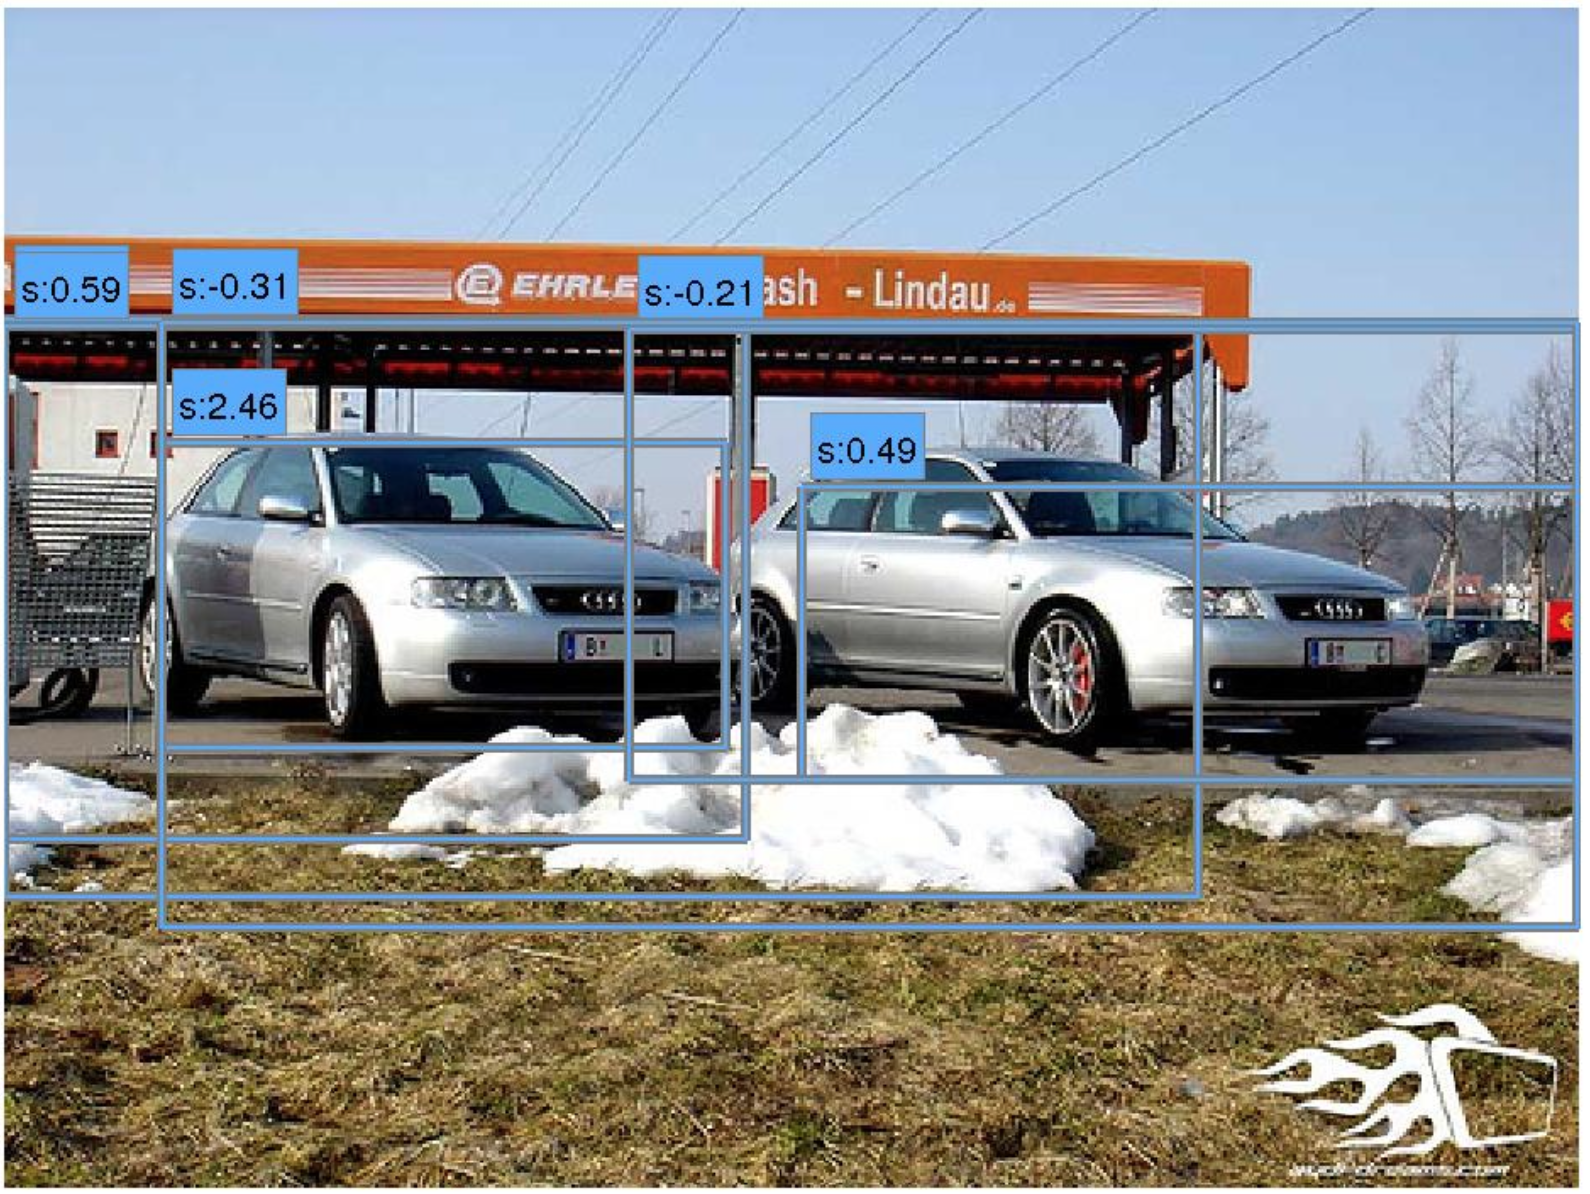
\includegraphics[width=0.24\textwidth]{car_cnn/2a.png} &   
          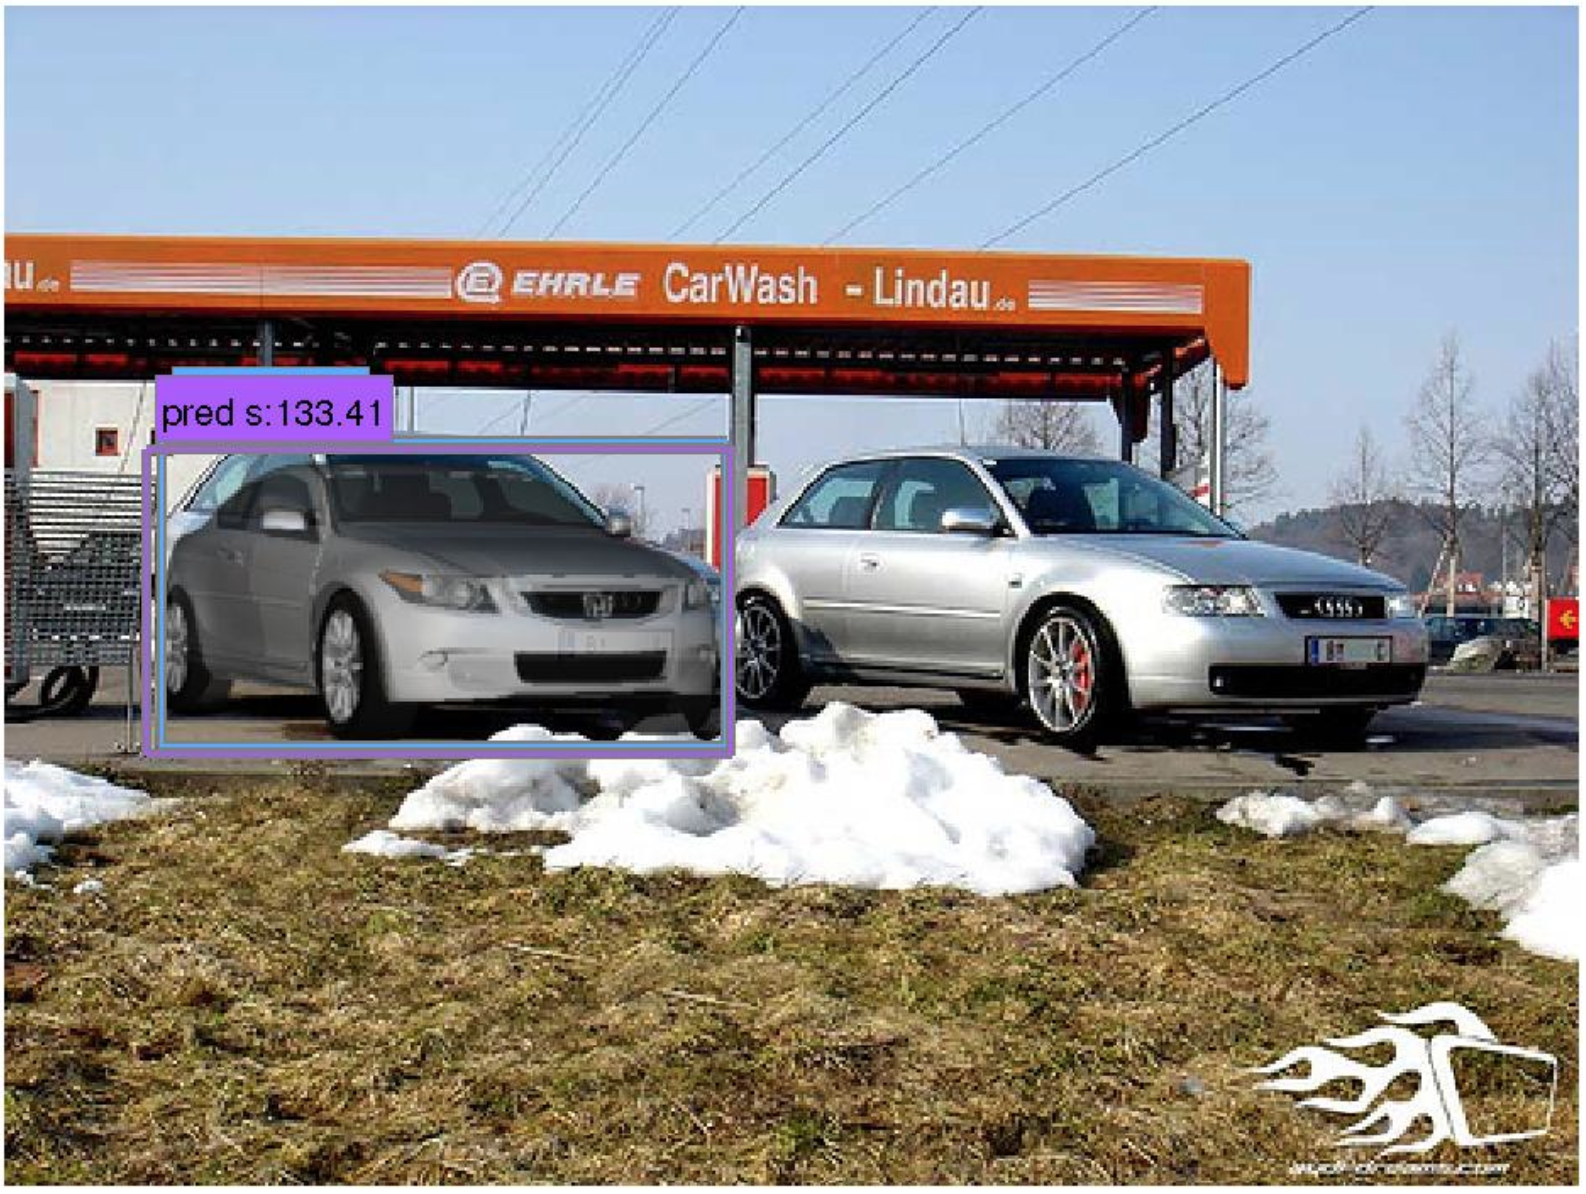
\includegraphics[width=0.24\textwidth]{car_cnn/2b.png} &   
          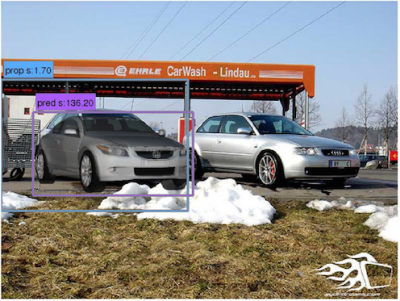
\includegraphics[width=0.24\textwidth]{car_cnn/2c.png} &   
          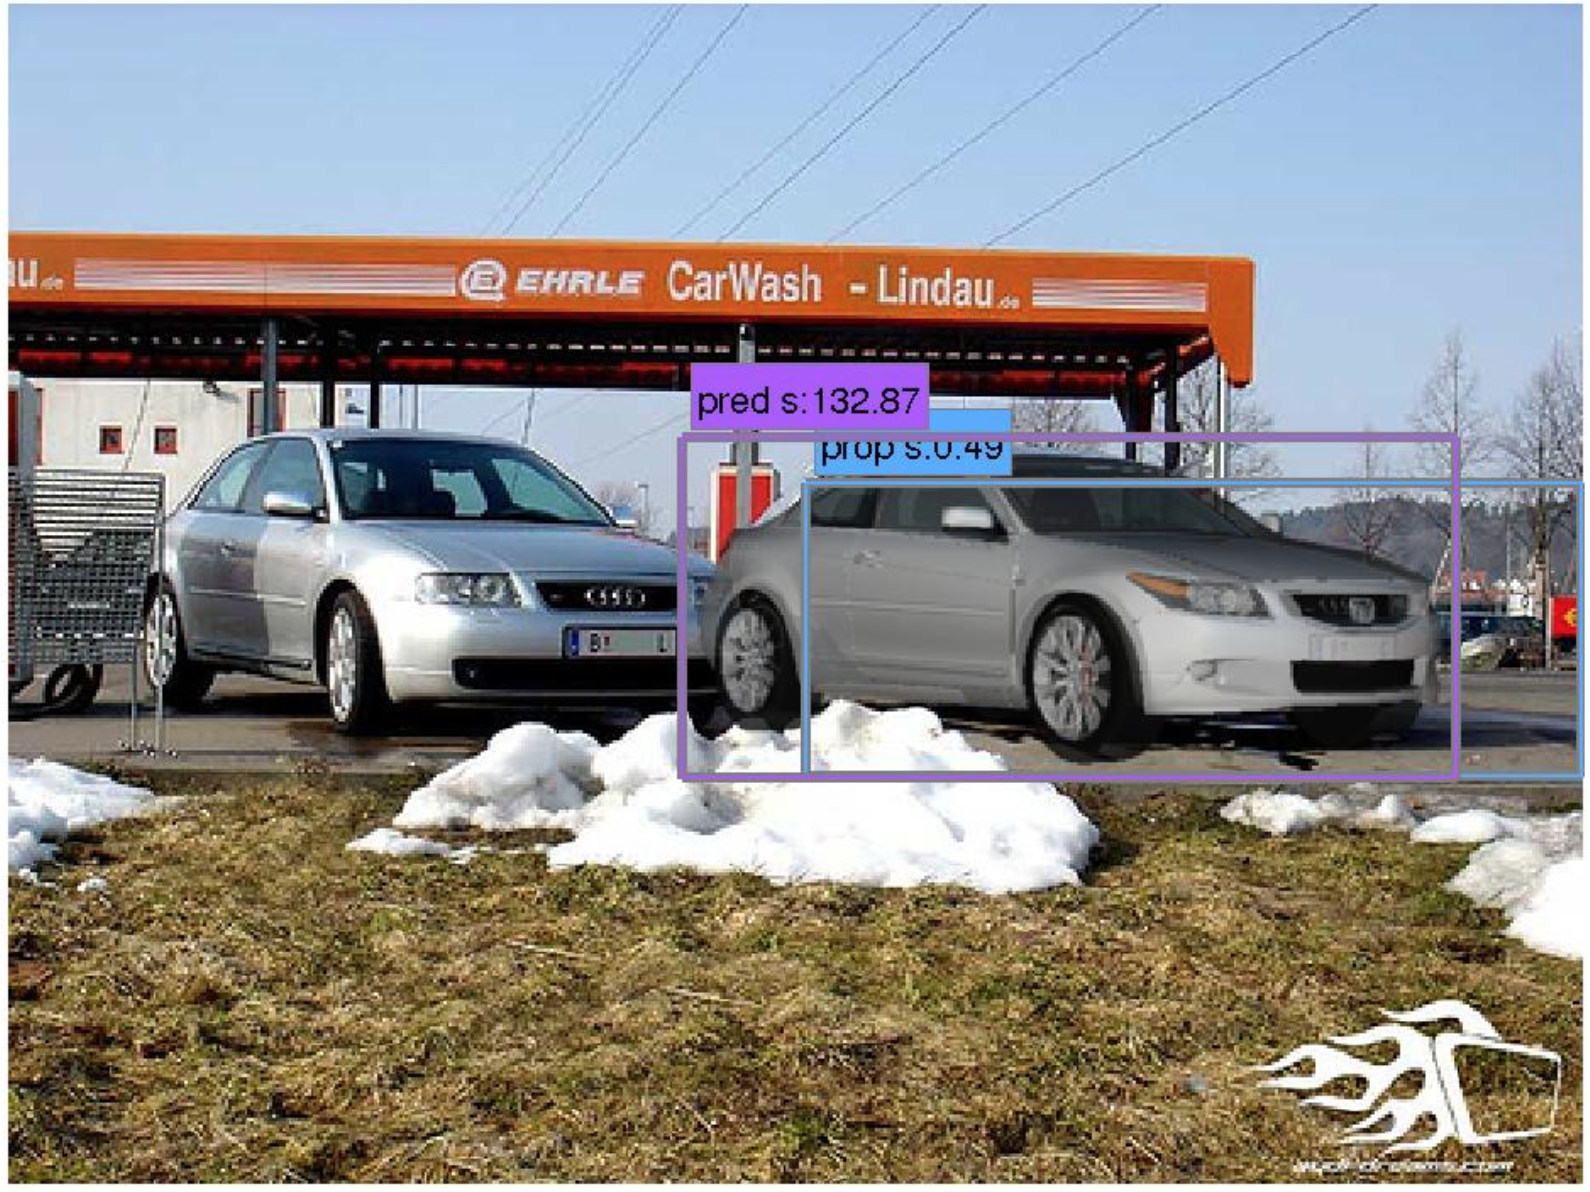
\includegraphics[width=0.24\textwidth]{car_cnn/2e.png}  \\  
          \hline
          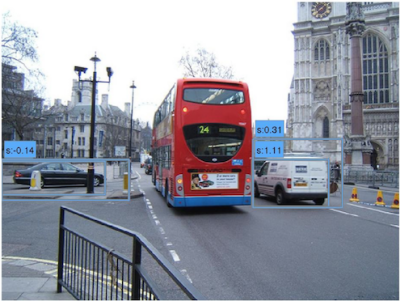
\includegraphics[width=0.24\textwidth]{car_cnn/4a.png} &   
          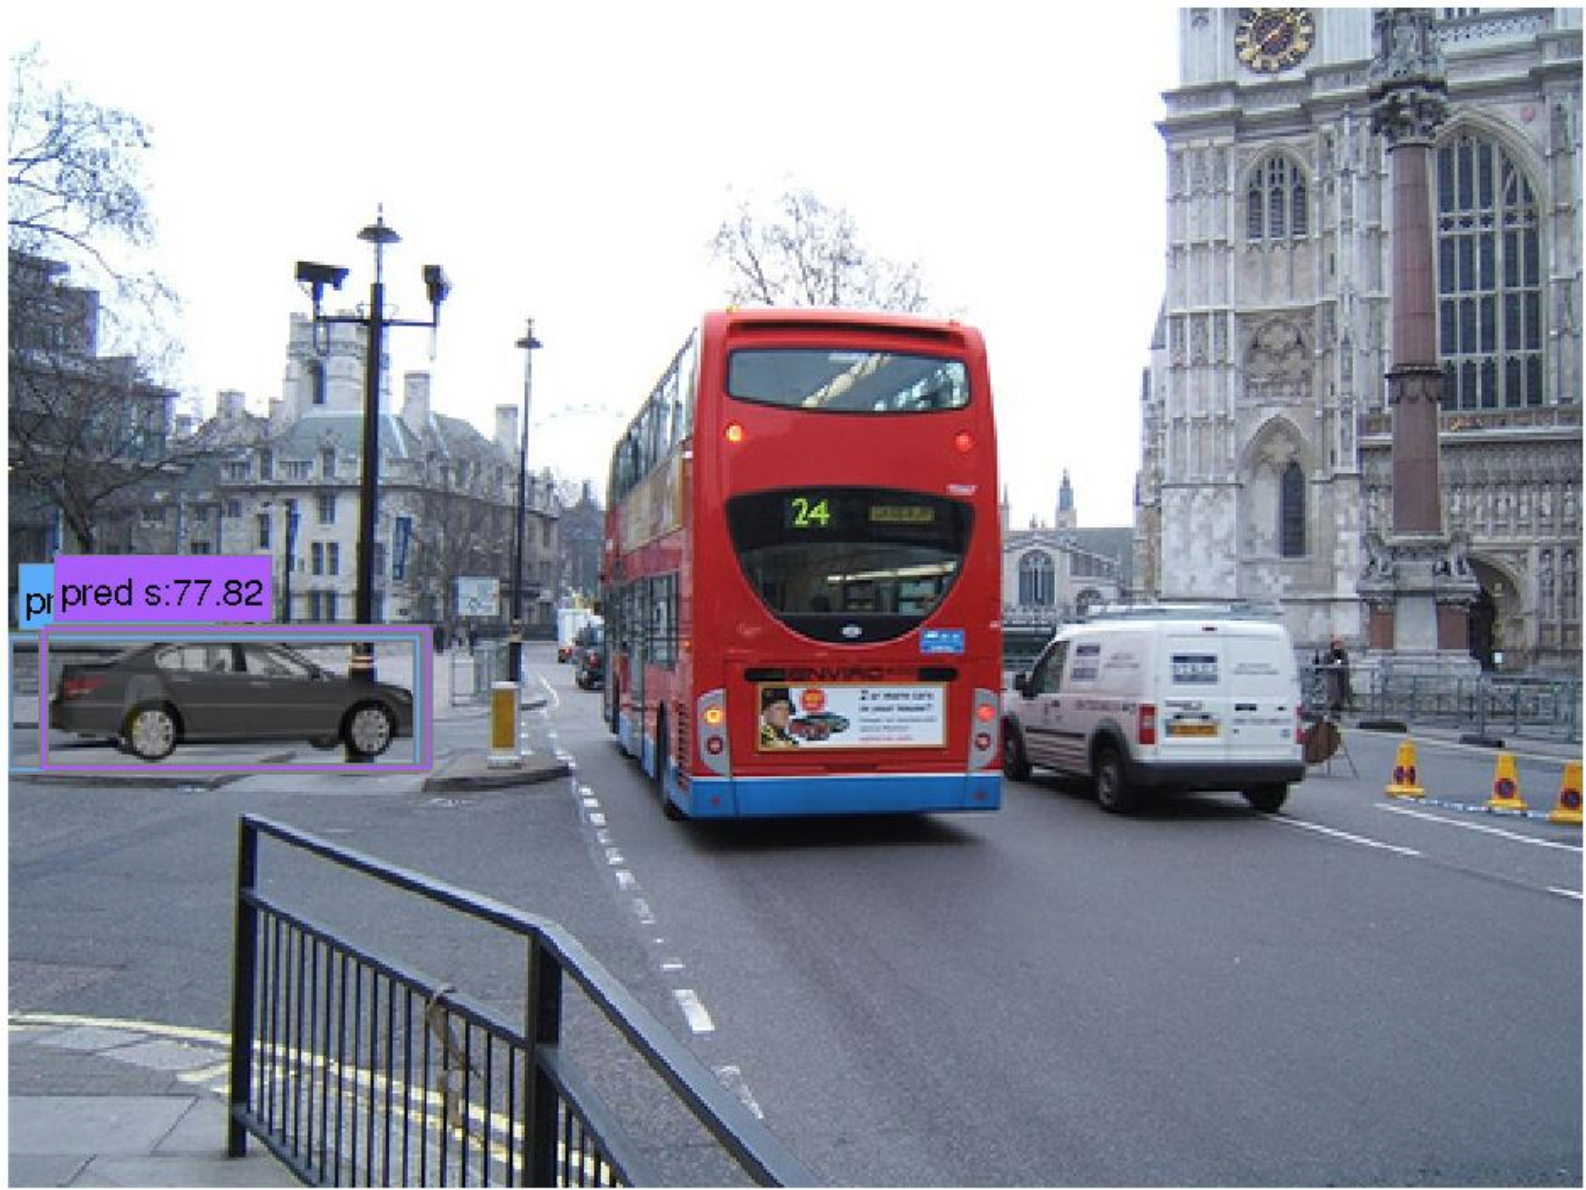
\includegraphics[width=0.24\textwidth]{car_cnn/4b.png} &   
          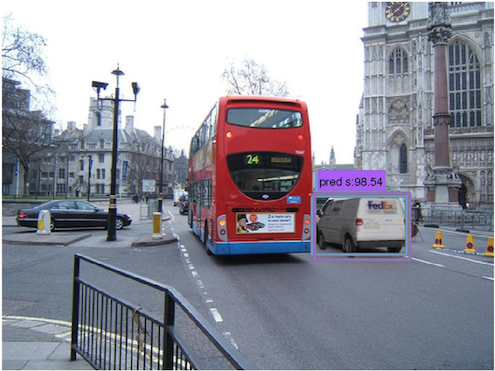
\includegraphics[width=0.24\textwidth]{car_cnn/4c.png} &   
          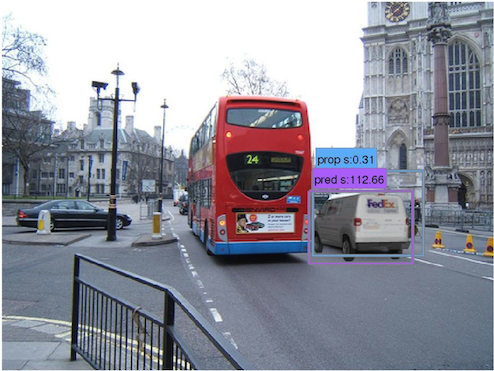
\includegraphics[width=0.24\textwidth]{car_cnn/4d.png}  \\  
        %    \hline
        %   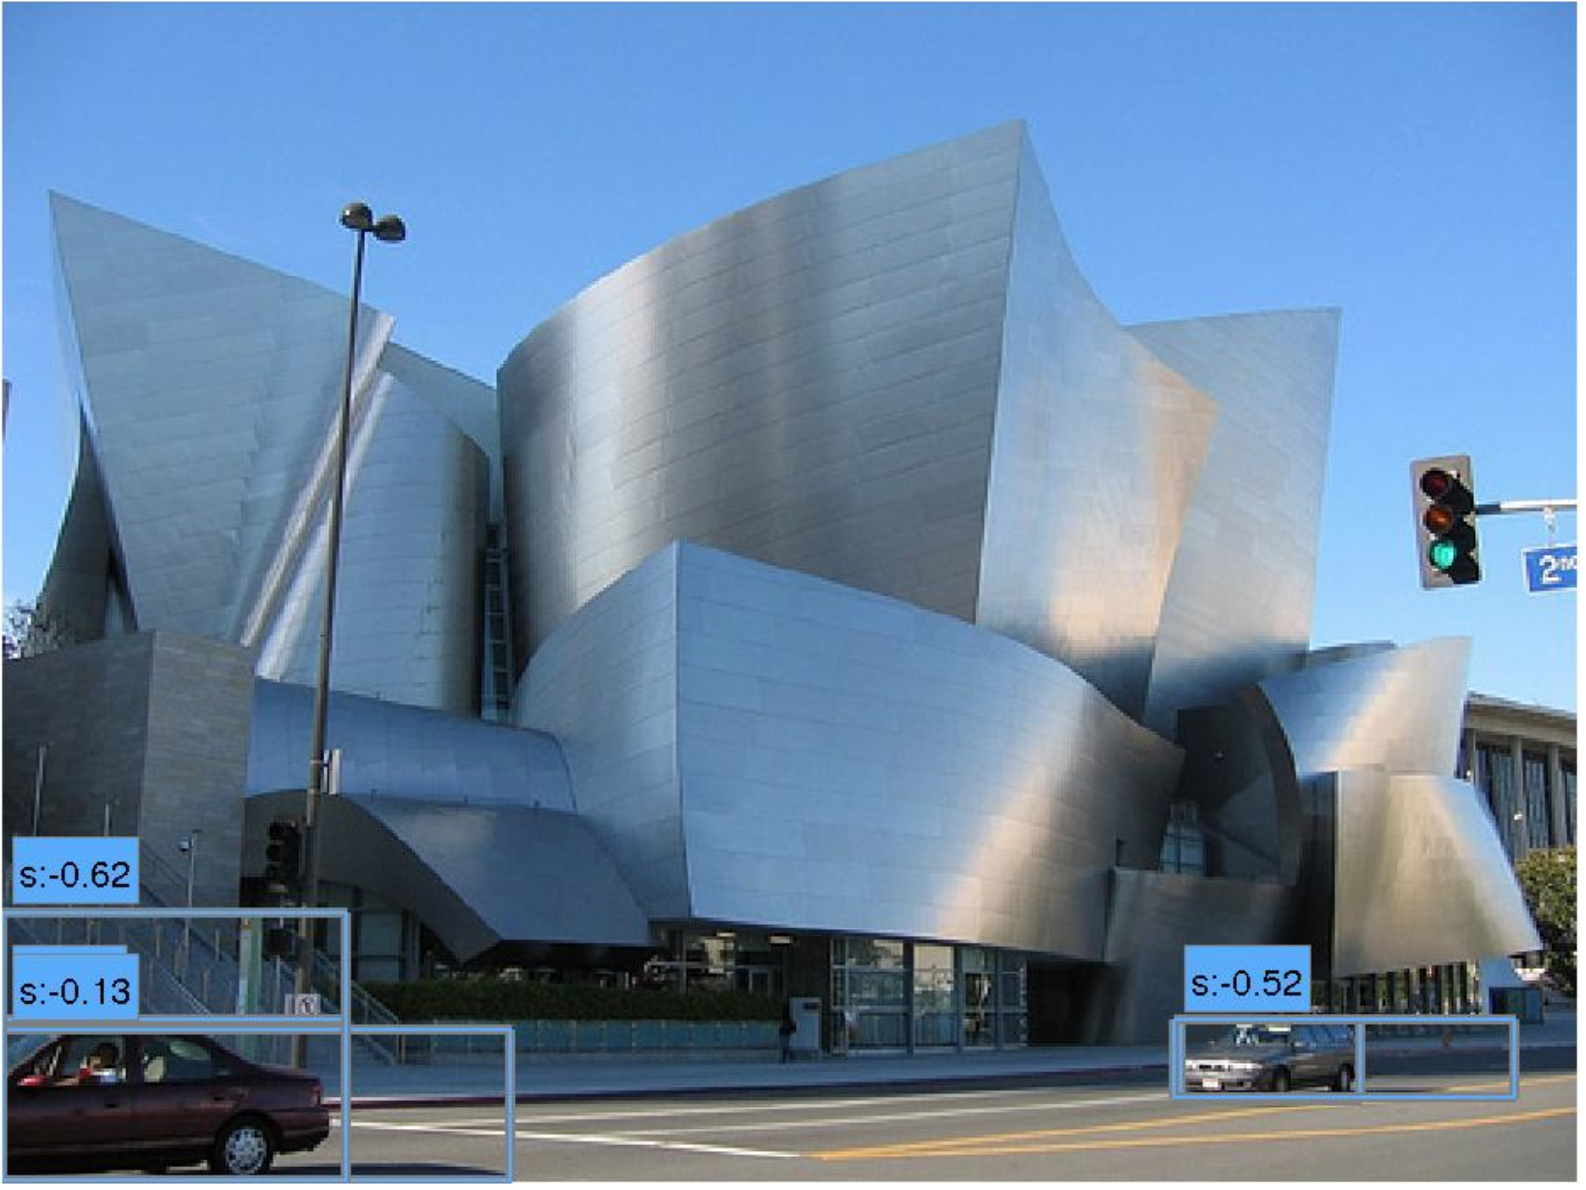
\includegraphics[width=0.24\textwidth]{car_cnn/10a.png} &   
        %   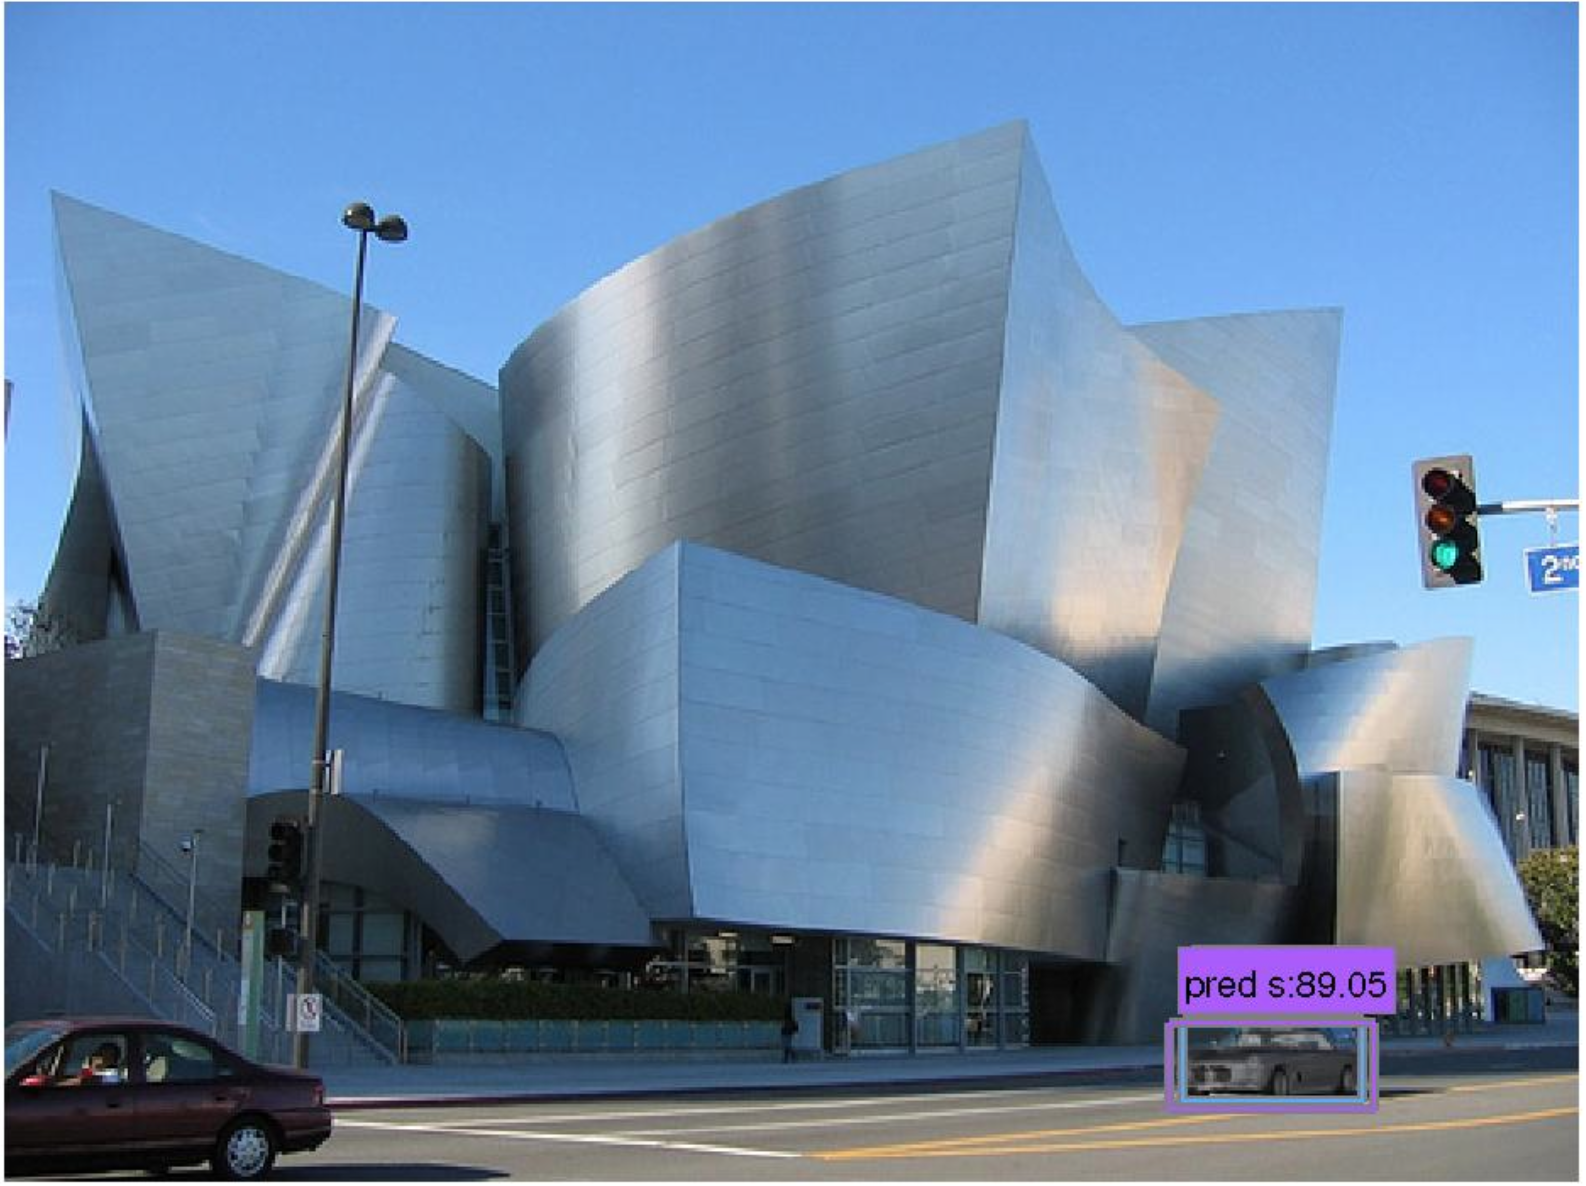
\includegraphics[width=0.24\textwidth]{car_cnn/10b.png} &   
        %   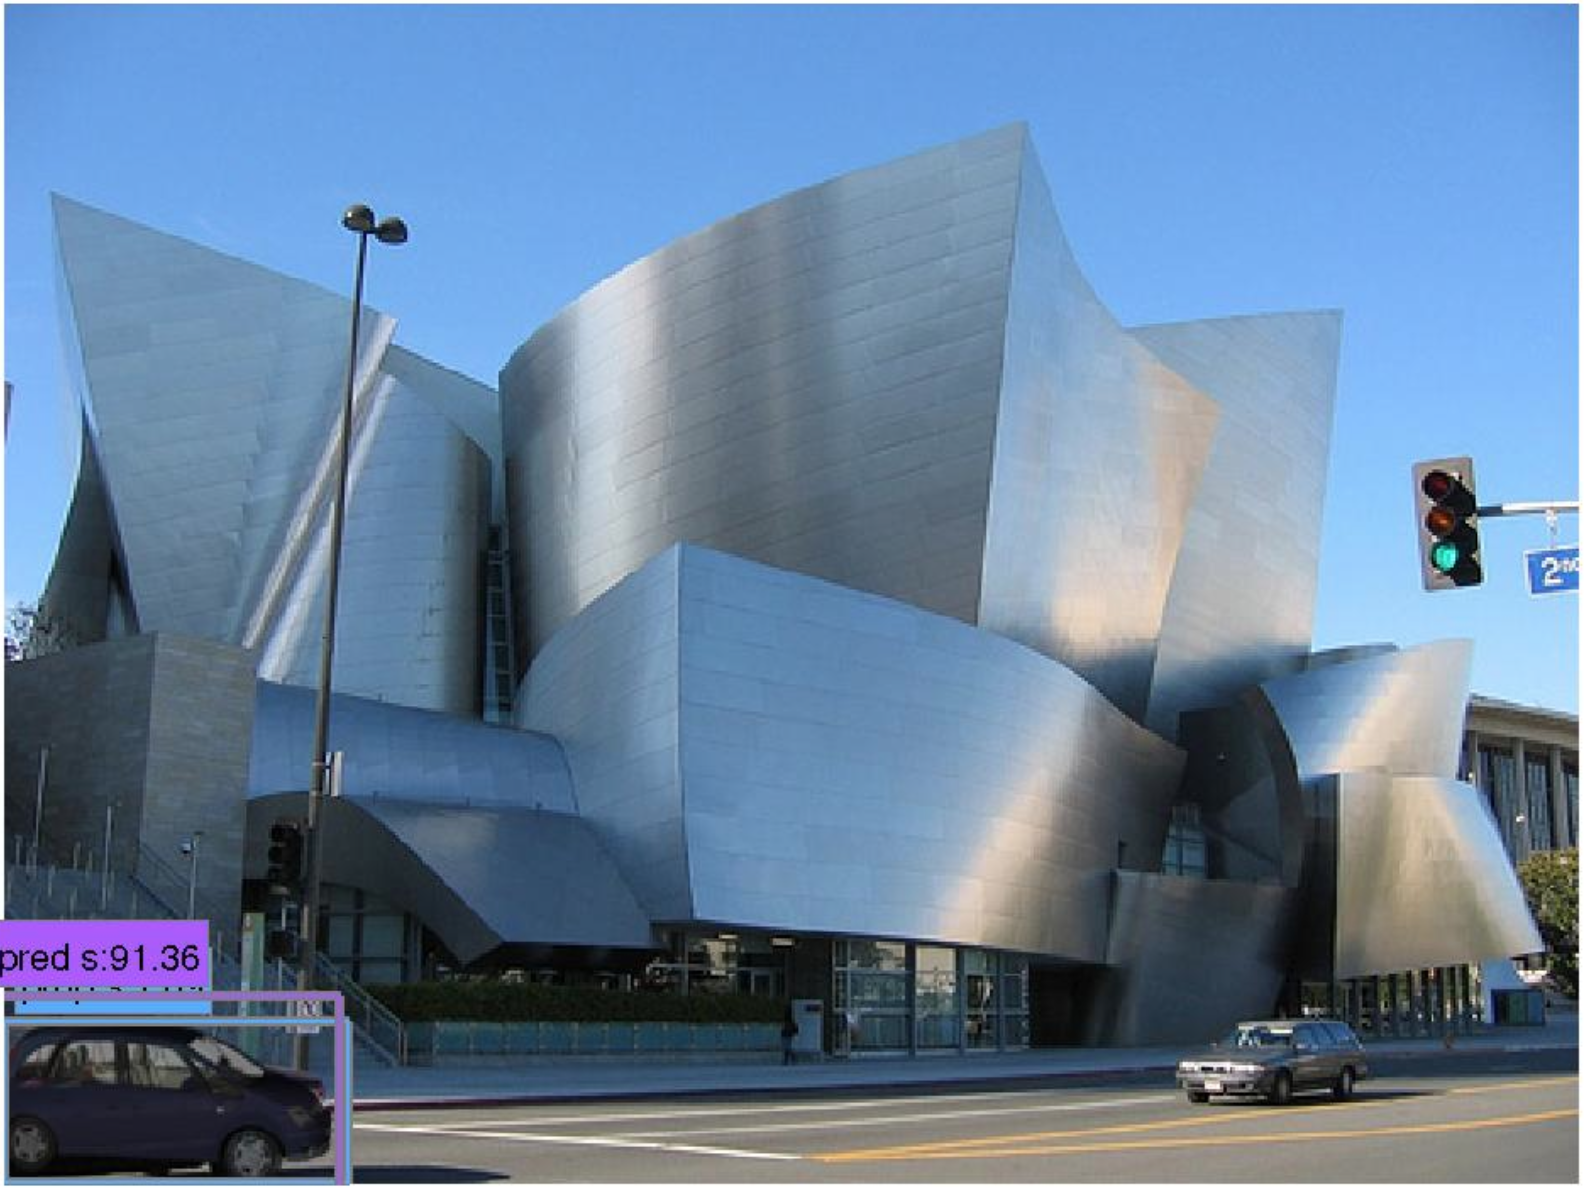
\includegraphics[width=0.24\textwidth]{car_cnn/10c.png} &   
        %   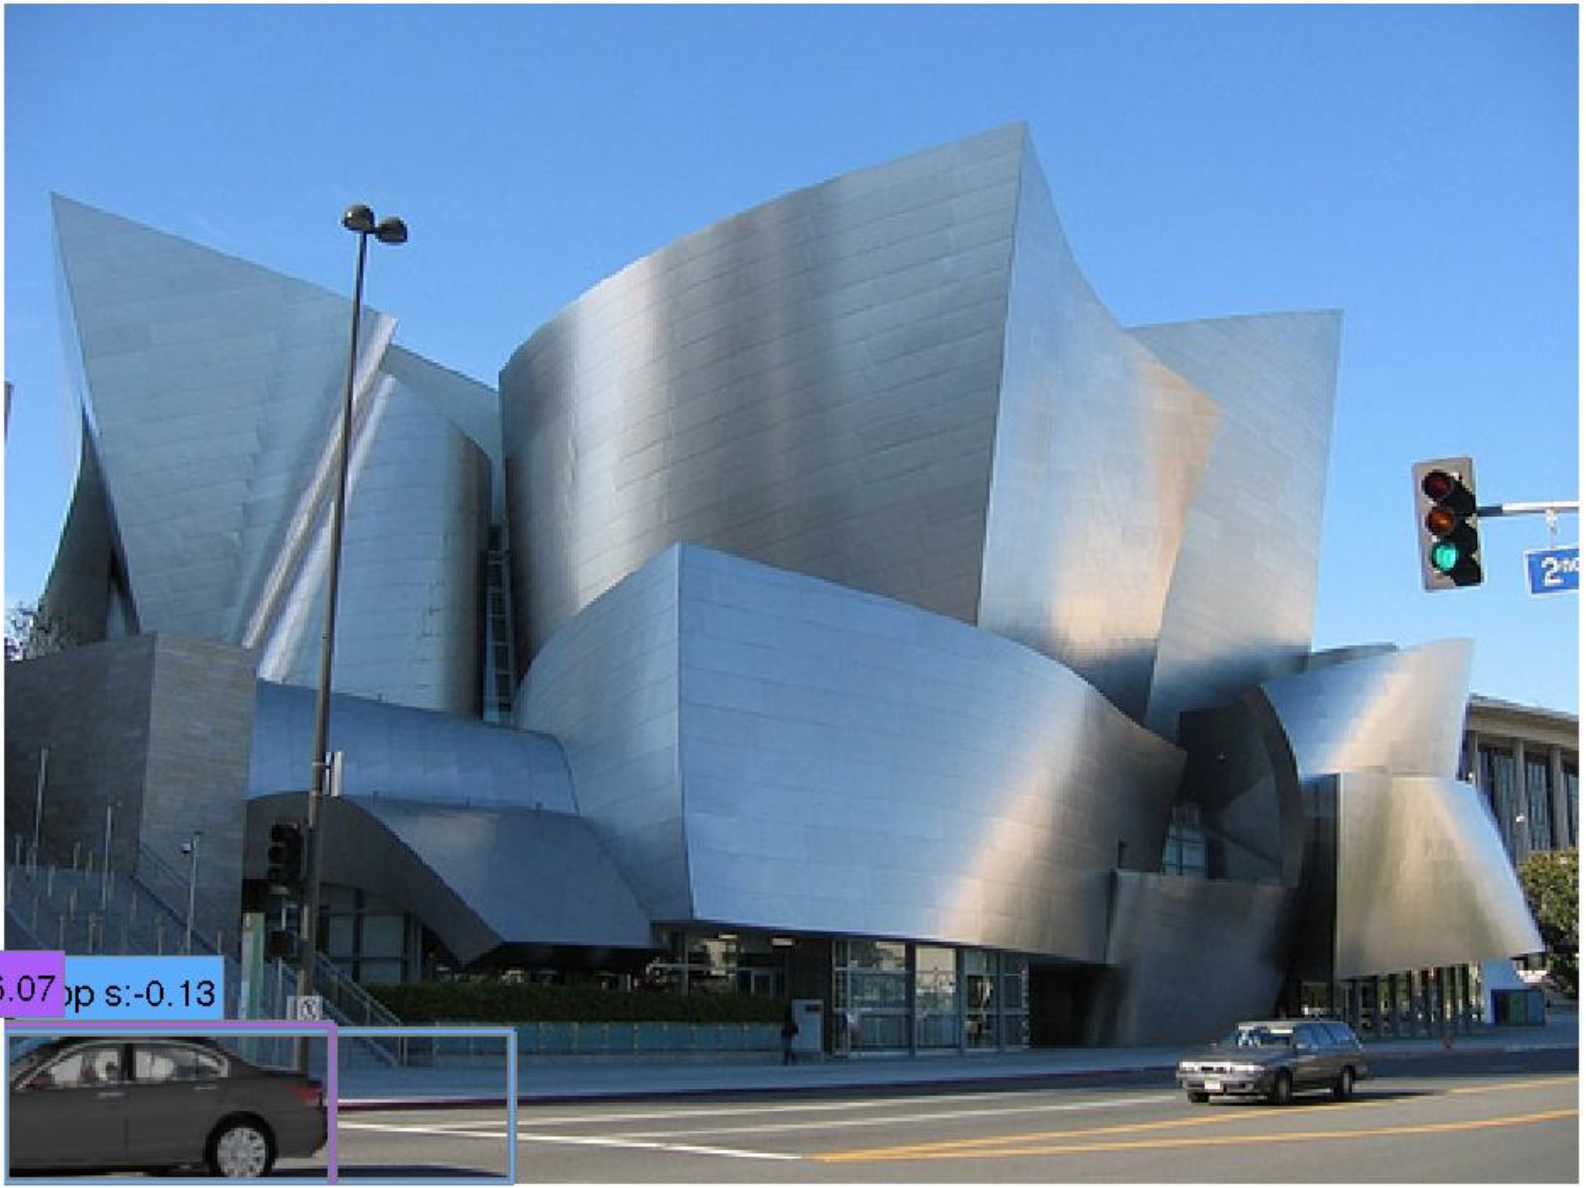
\includegraphics[width=0.24\textwidth]{car_cnn/10d.png}  \\  
        %   \hline 
        %   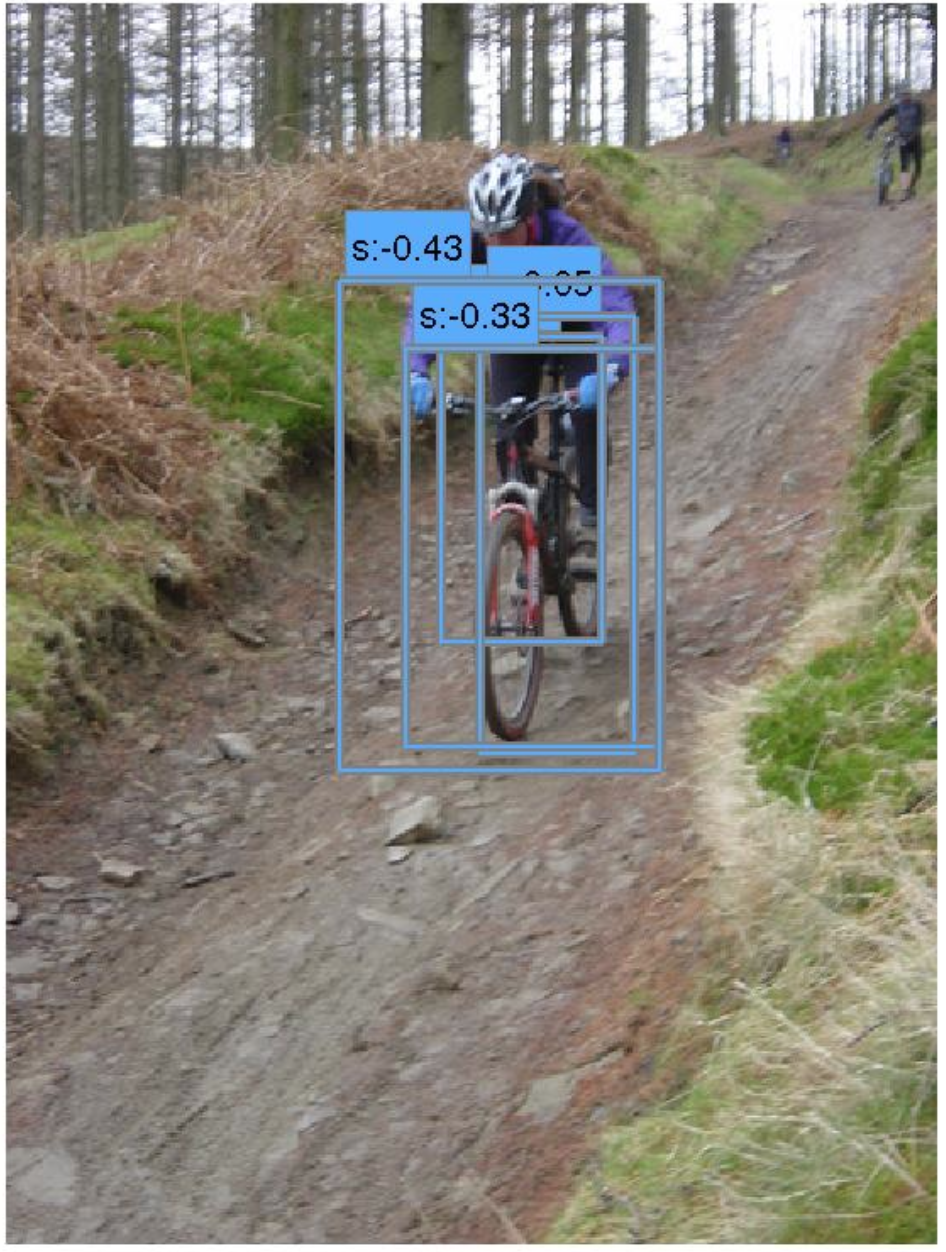
\includegraphics[width=0.24\textwidth]{bicycle_cnn/3a.png} &   
        %   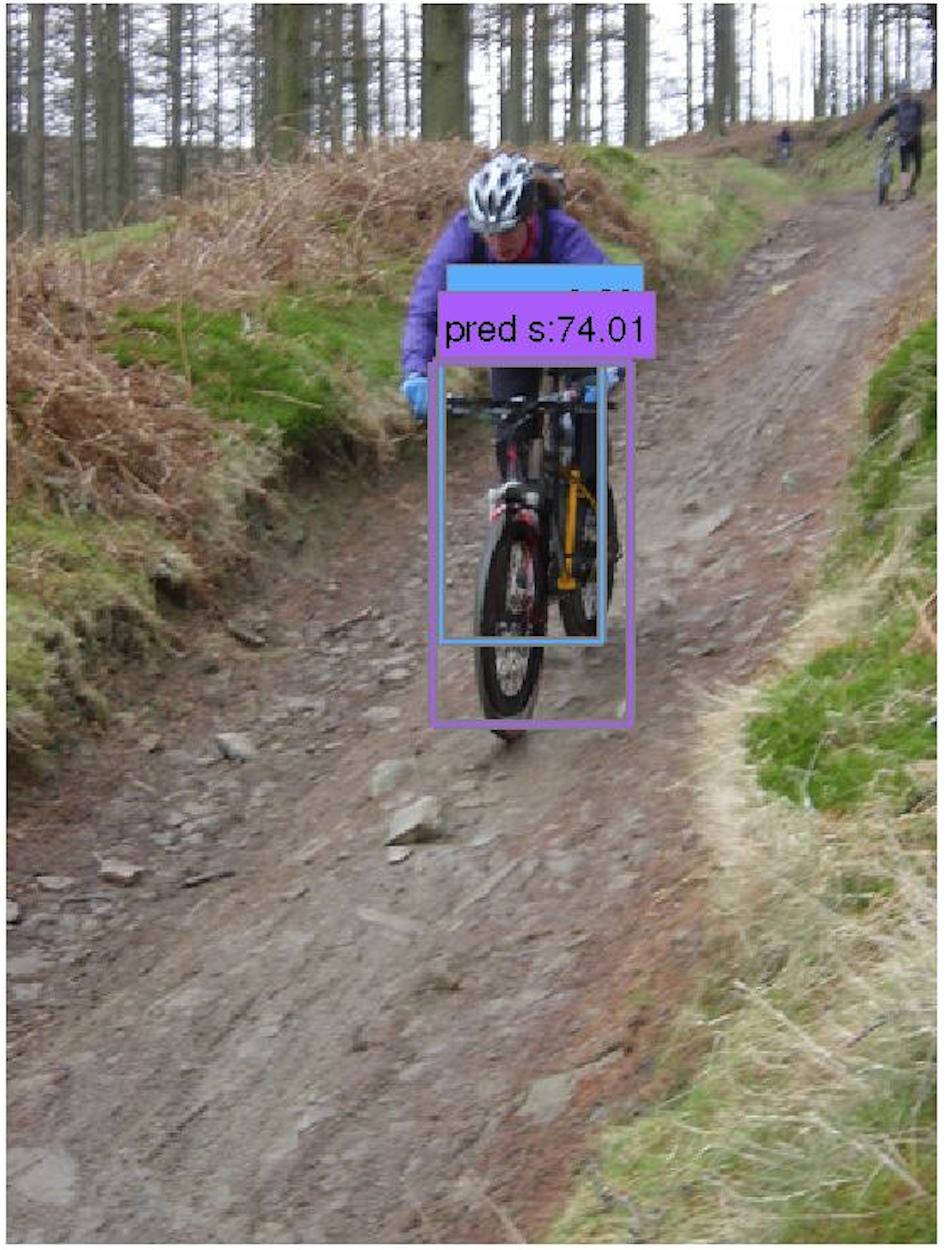
\includegraphics[width=0.24\textwidth]{bicycle_cnn/3b.png} &   
        %   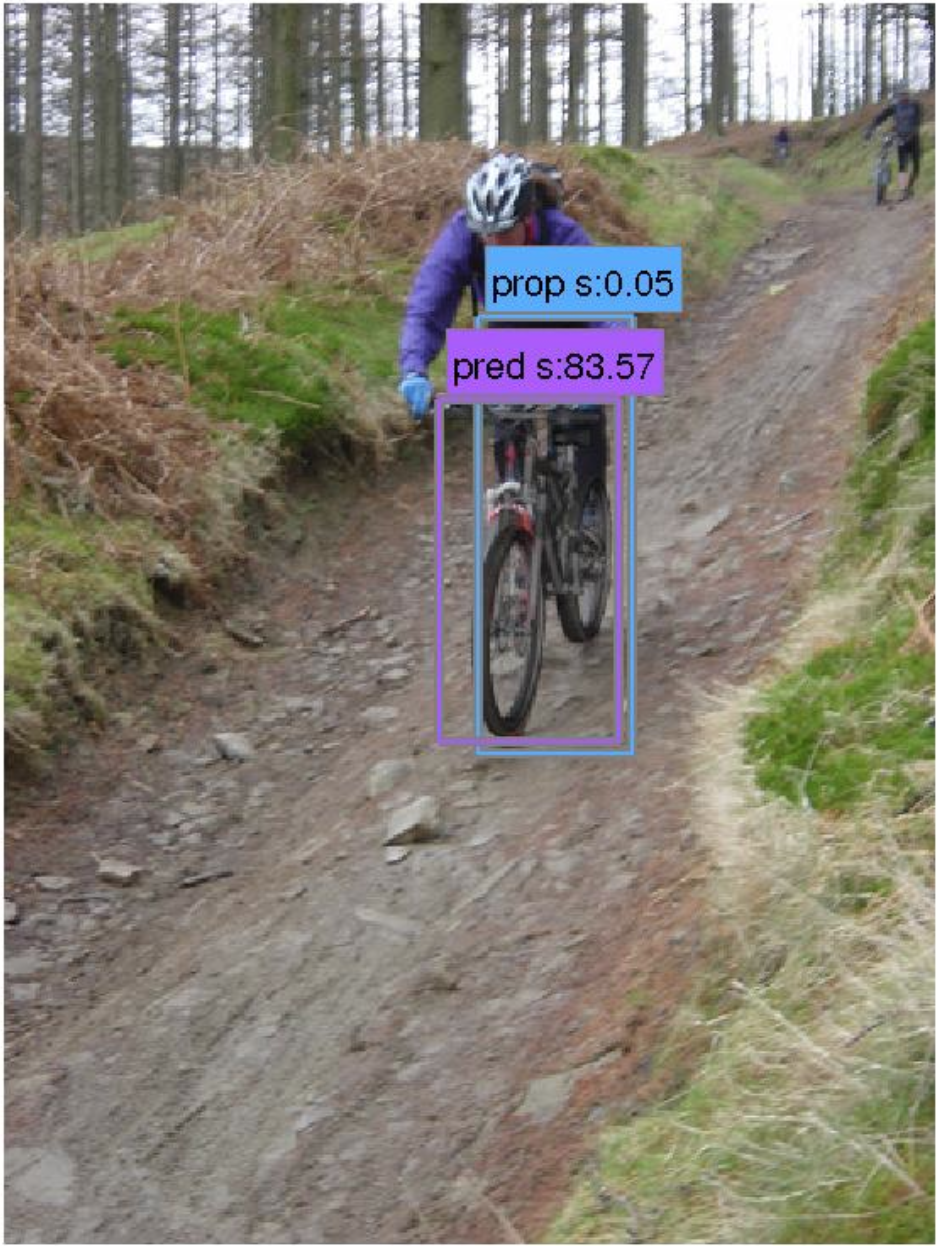
\includegraphics[width=0.24\textwidth]{bicycle_cnn/3c.png} &   
        %   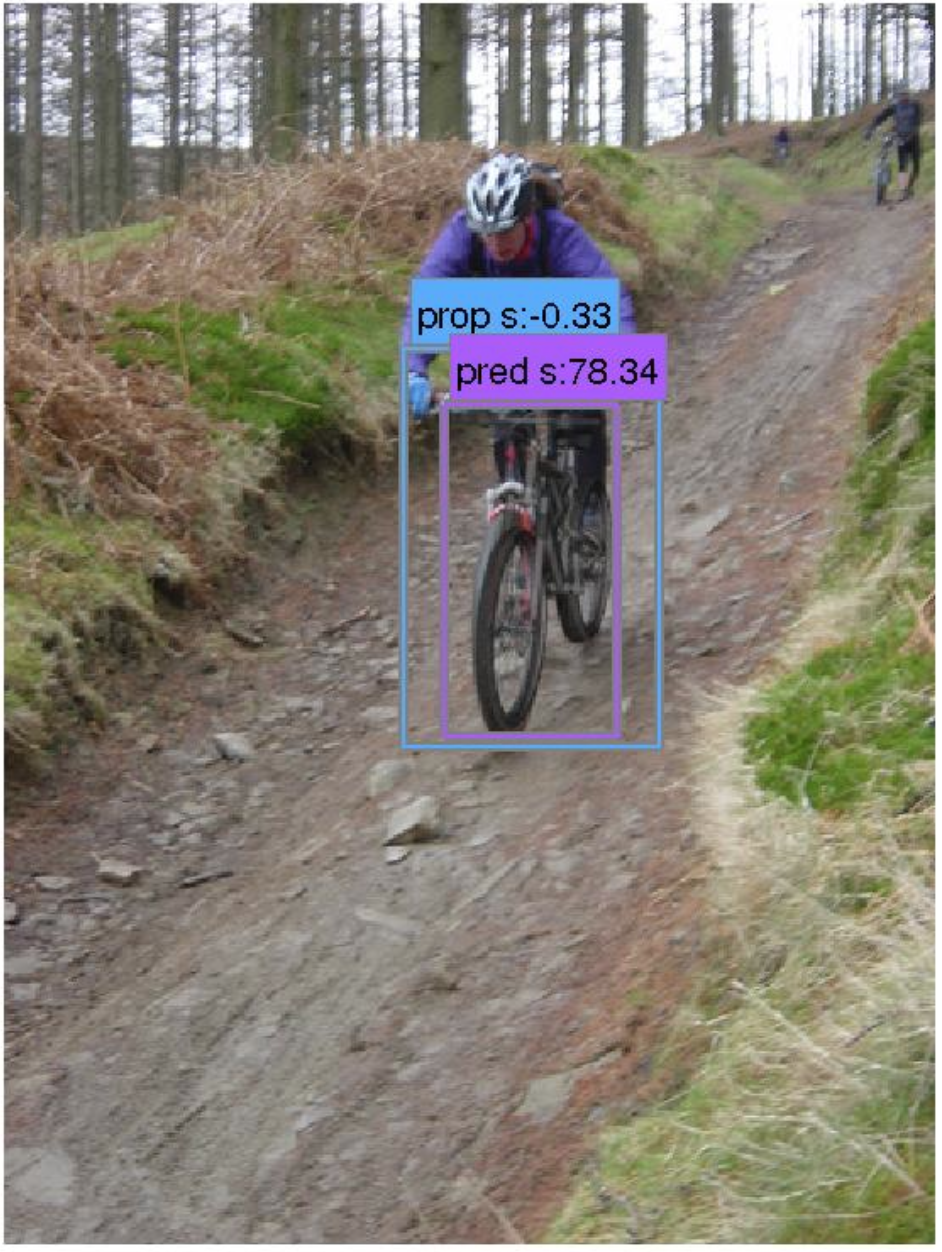
\includegraphics[width=0.24\textwidth]{bicycle_cnn/3d.png}  \\
        %
        % sorry no space
        %  \hline
        %  \includegraphics[width=0.24\textwidth]{bicycle_cnn/7a.png} &   
        %  \includegraphics[width=0.24\textwidth]{bicycle_cnn/7b.png} &   
        %  &\\
          \hline
          \includegraphics[width=0.24\textwidth]{bicycle_cnn/4a.png} &   
          \includegraphics[width=0.24\textwidth]{bicycle_cnn/4b.png} &   
          \includegraphics[width=0.24\textwidth]{bicycle_cnn/4c.png} &   
          \includegraphics[width=0.24\textwidth]{bicycle_cnn/4d.png}  \\
          \hline
          CNN Proposals & \multicolumn{3}{|c|}{Our matching results on proposal bounding boxes} \\
          \hline
        \end{tabular}
        \caption{Examples of enriched bounding boxes. Given R-CNN
            detection bounding boxes, our method predicted 2D-3D matching reasonably.
            Blue boxes are R-CNN output and purple boxes are the tightest
            bounding box enclosing predicted CAD model.}
          \label{fig:pascal12cnn}
        \end{figure}
        \vspace{-1.0em}
      \end{block}

      %-- Block 3-2
      \begin{block}{Conclusion}
        \begin{itemize}
          \item Non-Zero Whitened Histograms of Orientations (NZ-WHO)
            \begin{itemize}
              \item Generate E-LDA template from rendered 3D CAD data {\color{red} on-the-fly}
            \end{itemize}
          \item First attempt to simultaneously render and train exemplar detectors on-the-fly.
          \item Enrich the output of an existing object class detector
            \begin{itemize}
              \item 3D continuous pose and a 3D CAD model exemplar.
            \end{itemize}
        \end{itemize}
      \end{block}

      \begin{block}{Acknowledgement}
        \small
        We acknowledge the support of NSF CAREER grant (N1054127),
        Ford-Stanford Innovation Alliance Award, DARPA, Korea Foundation for
        Advanced Studies, Fulbright New Zealand and the Max Planck Center for
        Visual Computing \& Communication.
      \end{block}

      \begin{block}{References}
        {\footnotesize
        \bibliographystyle{../ieee}
        \bibliography{2349_poster}
        }
      \end{block}
    \end{column}%4
    
  \end{columns}
\end{frame}
\end{document}
